\documentclass[12pt,a4paper]{article}
\usepackage{longtable}
\usepackage[LGR,T1]{fontenc}
\usepackage{lscape}
%\usepackage{pdfsync}
\usepackage{multirow}
\usepackage{amsmath,bm} 
\usepackage{amsfonts}
\usepackage{amsthm} % Extended theorem environments
%\usepackage{amssymb} % Math symbols %%redundant with stix package
%\usepackage{esint} % Intégrales multiples
%\usepackage{esvect} % Vecteurs
\usepackage{mathtools}
\usepackage{pifont} 
\usepackage[version=4]{mhchem} % Chemical equations
 
\usepackage{fancyhdr}
\usepackage{graphicx}

\graphicspath{{../frontend/img/}{../chap_intro_ccl/img/}{../chap_case_study/img/}{../chap_ES_PCE/img/}{../chap_electro_uq/img/}{../chap_methodo/img/}{../chap_myopic/img/}{../chap_RL/img/}{../chap_atom_mol/img/}{../chap_RobPol/img/}{../appendices/img/}{../rebuttals/img/}} % Figures folder different for each input
%\graphicspath{{img/}} %
\DeclareGraphicsExtensions{.eps,.pdf,.png,.jpg}




\usepackage{lastpage}
\usepackage{afterpage}
\usepackage{lettrine}
\usepackage{color,soul}
\usepackage[dvipsnames]{xcolor}
\usepackage{colortbl}
\usepackage{enumitem}
\usepackage{tikz}
\usepackage{titlesec}
\def\eg{e.g.,\ }
\def\ie{i.e.,\ }

\newcommand{\clearemptydoublepage}{\newpage{\pagestyle{empty}\cleardoublepage}} %pour effacer les en-tetes sur la page vierge avant chaque chapitre


%Palatino font
%\usepackage{pxfonts}
%\usepackage{libertine}
\usepackage[scaled=0.88]{beraserif}
\usepackage[scaled=0.85]{berasans}
\usepackage[scaled=0.84]{beramono}
\usepackage{mathpazo}
%\linespread{1.05}
\usepackage[T1,small,euler-digits]{eulervm}

\usepackage[nomessages]{fp}


\definecolor{bleuUCLclair}{rgb}{.09, 0.569, 1}
\definecolor{bleuUCLfonce}{rgb}{ .13, .52, .86}
\definecolor{redBurn}{rgb}{.91, 0.29, 0.08}

\usepackage{tocloft}

%\renewcommand{\cftsecpresnum}{Reviewer \#}
\renewcommand{\cftsecpresnum}{}
\renewcommand{\cftsecnumwidth}{6em}
\renewcommand{\cftsubsecpresnum}{}
\renewcommand{\cftsubsecnumwidth}{6em}

\setcounter{tocdepth}{3}
\setcounter{secnumdepth}{3}

\usepackage[nottoc]{tocbibind}
\usepackage[colorlinks=true,urlcolor=black,linkcolor=black,citecolor=black]{hyperref}
\usepackage[square,numbers,sort&compress]{natbib}

\bibliographystyle{biblio/elsarticle-num-names}  %Ordered by appearance in the text, with DOI and URL
%\usepackage[backend=biber, natbib=true, style=numeric-comp, citestyle=numeric-comp, sorting=none, giveninits=true, maxcitenames=1]{biblatex}

\usepackage[]{tocbibind}
\usepackage{hyperref}
\hypersetup{
    colorlinks=true,
%    linkcolor=black,
    bookmarks=true,
    pdfpagemode=FullScreen,
}
\setcounter{tocdepth}{2}

\addtolength{\topmargin}{-1.5cm}
\addtolength{\textheight}{1.5cm}
\addtolength{\textwidth}{2cm}
\addtolength{\footskip}{2cm}
\setlength{\evensidemargin}{-0.5cm}
\setlength{\oddsidemargin}{-0.5cm}
\setlength{\arrayrulewidth}{0.25pt}

\renewcommand{\baselinestretch}{1.1} % Interligne


\newenvironment{maliste}%
{ \begin{list}%
	{\textcolor{bleuUCLfonce}{$\bullet$}\hspace{0.5cm}}%
	{\setlength{\labelwidth}{50pt}%
	 \setlength{\leftmargin}{25pt}%
	 \setlength{\itemsep}{30pt}}}%
{ \end{list} }

%\renewcommand{\headrulewidth}{0.0pt}
%\newcommand{\clearemptydoublepage}{%
%	\newpage{\pagestyle{empty}\cleardoublepage}}




%section like title in longtable
\newcommand{\seclong}[1]{\multicolumn{2}{@{}l}{{\Large\sffamily #1}} 
\vspace{0.5cm}
\\}

%enumerate on two columns
\newcounter{listlong}
\newcommand{\newlistlong}{\setcounter{listlong}{1}}
\newcommand{\iteml}[1]{%
\hspace{4.5cm}\textcolor{redBurn}{\arabic{listlong}}\stepcounter{listlong}%
&%
#1%
 
\\%
}

%left in column
\newcommand{\lcol}[1]{%
\begin{minipage}[t]{.35\textwidth}%

#1%

\end{minipage}%
}

\title{\vspace{-1cm}
\begin{flushleft} {\sffamily Xavier Rixhon's PhD thesis - Answers to jury members}\end{flushleft}}
\date{\vspace{-1.7cm}\begin{flushleft}\sffamily Exploration of uncertainty-aware energy transition pathways - Reinforcement learning and principal component analysis-based methods\end{flushleft}}
%
%Xavier Rixhon, Gauthier Limpens, Diederik Coppitters, Hervé Jeanmart and Francesco Contino\end{flushleft}}


\pagestyle{fancy} 
\fancyhf{}
\fancyfoot[R]{\sffamily\thepage\ / \pageref{LastPage}}
  \fancyfoot[L]{ }

\fancypagestyle{plain}{%
  \fancyhf{}%
  \fancyfoot[R]{\sffamily\thepage\ / \pageref{LastPage}}
  \fancyfoot[L]{ }
}

\renewcommand{\headrulewidth}{0.0pt}


\newcommand{\hlc}[2][yellow]{ {\sethlcolor{#1} \hl{#2}} }

\titleformat{\section}
  {\bfseries\scshape}{}{1em}{}

\titleformat{\subsection}
  {\normalfont\scshape}{}{1em}{}

\usepackage[framemethod=default]{mdframed}
%\mdfsetup{skipabove=\topskip,skipbelow=\topskip}

\global\mdfdefinestyle{comment}{%
     linecolor=red,linewidth=0.1cm,%
     leftmargin=-0.5cm,rightmargin=-0.5cm, innerleftmargin=0.4cm,innerrightmargin=0.4cm,
     topline=false,bottomline=false
}

\global\mdfdefinestyle{manuscript}{%
     linecolor=gray!20,linewidth=0.05cm,backgroundcolor=gray!20,%
     leftmargin=-0.5cm,rightmargin=-0.5cm, innerleftmargin=0.4cm,innerrightmargin=0.4cm
}
  
  \renewcommand{\subsectionautorefname}{Comment}
\begin{document}
\maketitle

I would like to thank the jury members for the comments, which significantly helped improving the manuscript and substantiating the novelty of my work. Based on the notes taken during the private defense, I hereby transcribed, as accurately as possible, the jury's comments. 

I believe I have addressed all the issues raised in the following answers. Some of them required adaptations of the text. These adaptations are either directly in the thesis manuscript or left for further developments in subsequent papers. For each comment, I have first highlighted the issue, then provided an answer, and finally described how the manuscript was adjusted, if needed.\\

When a comment explicitly comes from specific members of the jury, they are listed at the beginning of the comment with the following color code: {\color{orange} \textbf{Stefano} Moret}, {\color{teal} \textbf{Stefan} Pfenninger}, {\color{purple} \textbf{Sylvain} Quoilin} and {\color{violet} \textbf{Christophe} De Vleeschouwer}. Here is how an answer to a comment is structured:

\begin{mdframed}[style=comment] % Comment from the reviewer
Text of the comment. When a page number is mentioned at the beginning of the comment, it refers to the page number of the manuscript submitted before the private defense, which might differ from the one in its final version.
\end{mdframed}

\noindent The answer provided to the comment and, based on this, where the potential modification brought to the manuscript is located in the thesis manuscript using {\color{blue} blue font}.

\begin{mdframed}[style=manuscript] % Modification brought to the manuscript
New version of the text in the manuscript.
\end{mdframed}

% {\color{orange} \textbf{Stefano}}
% {\color{purple} \textbf{Sylvain}}
% {\color{teal} \textbf{Stefan}}
% {\color{violet} \textbf{Christophe}}

\clearpage
%\tableofcontents
%
%\clearemptydoublepage

\section{General comments/questions}
\label{General}

\begin{mdframed}[style=comment] % Comment from the reviewer
{\color{orange} \textbf{Stefano}} - Overall, many methods: PCE + RL + NN + PCA. At each stage, some assumption is made. Why not a simpler approach or a simpler model? Do you need all these steps? Explain the role of the different methods and why PCE instead of monthly version for uncertainty? 
\end{mdframed}

\noindent

\begin{mdframed}[style=manuscript] % Comment from the reviewer

\end{mdframed}

\begin{mdframed}[style=comment] % Comment from the reviewer
{\color{violet} \textbf{Christophe}} - The variables and the uncertainties should be presented in a compact and mathematical way.
\end{mdframed}

\noindent In my opinion, the main variables of EnergyScope Pathway are presented {\color{blue} in Section 1.1 of the core of the manuscript}. Further details are also given {\color{blue}in Appendix B.2}. Finally, these variables are even exhaustively detailed in \cite{limpens2019energyscope} and \cite{limpens2024pathway} that are cited several times in the thesis manuscript.  Regarding the uncertainties, the way the ranges are defined and the way they affect the value of some parameters in the model are explained {\color{blue}in Section 1.2 of the core of the manuscript}. Consequently, no modification has been brought to the manuscript regarding this topic.

\subsection{Assumptions - Fine tuning}
\label{fine_tuning}

\begin{mdframed}[style=comment] % Comment from the reviewer
{\color{orange} \textbf{Stefano}}, {\color{purple} \textbf{Sylvain}} \& {\color{teal} \textbf{Stefan}} - Many assumptions, e.g., alpha = 85\% (p. 40) or reward = -300 (Chapter 4). How sensitive are the results to these assumptions? It looks like all these parameters have been tuned to obtain the desired results. How robust are they? Can the methodology be generalized to other models? Can we keep the same values for other applications? You need a model that runs pretty fast, right?
\end{mdframed}

\noindent Perhaps there is a need to better prove or show that it is not a magic number.  How to generalise it and hook it to something physical (even if it is done a posteriori). Guidelines to apply it to some other models

\begin{mdframed}[style=manuscript] % Comment from the reviewer

\end{mdframed}

\begin{mdframed}[style=comment] % Comment from the reviewer
{\color{purple} \textbf{Sylvain}} - Make sure to discuss the hypotheses because one might not agree with all of them. So, it could provide more context but also some limitations and indications of the alternatives (and the spectrum of what is possible).
\end{mdframed}

\noindent

\begin{mdframed}[style=manuscript] % Comment from the reviewer

\end{mdframed}



\subsection{Graphs and results}
\label{general_graphs_results}

\begin{mdframed}[style=comment] % Comment from the reviewer
{\color{orange} \textbf{Stefano}} - Work on the graph of slide 19 (there is a misunderstanding on the fact that the grey curve is labelled as failure but they are failures in the future)
\end{mdframed}

\noindent To clarify this point, I have extended the caption of the related figures (see previous comments) and added two sentences in {\color{blue} Section 4.2.2}:

\begin{mdframed}[style=manuscript] % Comment from the reviewer
Since infeasible cases or those that overshoot the \ce{CO2}-budget are discarded before reaching 2050 (see Section 4.1.2), the number of attempts that reach further steps in the transition progressively decreases. Consequently, the share of successful transitions compared to failures progressively increases with time. 
\end{mdframed}

\begin{mdframed}[style=comment] % Comment from the reviewer
{\color{orange} \textbf{Stefano}}, {\color{teal} \textbf{Stefan}} \& {\color{purple} \textbf{Sylvain}} - Graphs like the ones presented during the private defense (slides 22 and 24) should be better explained. In general, improve the presentation of the results, especially for the RL chapter.
\end{mdframed}

\noindent 

\begin{mdframed}[style=manuscript] % Comment from the reviewer

\end{mdframed}

\begin{mdframed}[style=comment] % Comment from the reviewer
{\color{orange} \textbf{Stefano}}, {\color{teal} \textbf{Stefan}} \& {\color{purple} \textbf{Sylvain}} - Many axes labels are missing, and the captions are often insufficient to read the figures. 
\end{mdframed}

\noindent I agree and have gone through all the figures of the manuscript to clarify them by adding axes labels or extending the caption where it was needed. Figures where y-axis (and its label) is missing are distribution (or density) plots (\ie Figures 3.6, 4.4, 4.5, 4.6, 4.8 and E.1).  Consequently, similarly to an histogram, the feature of interest and its span of values are represented on the x-axis. The y-axis has no real interest in terms of information. What matters is the shape of the curve to be able to point out for which values/ranges of values, the feature of interest occurred more or less often.  For this reason, I have not added y-axis for the aforementioned figures but rather improved their respective caption, emphasising, among other things, that these figures represent distribution of occurrences. For instance, the caption of {\color{blue}Figure 4.4} is now more explicit:

\begin{mdframed}[style=manuscript] % Comment from the reviewer
Exploration of the state space over the learning process: distribution of occurrence of cumulative emissions (left) and costs (right). Number of remaining attempts decrease with time since infeasible problem and solutions overshooting the \ce{CO2}-budget are discarded prematurely, \ie before reaching 2050. Distributions labelled as ``Failure'' represent the attempts that overshot the \ce{CO2}-budget by 2050 at the latest. The majority of successful transitions have cumulative emissions much lower than the \ce{CO2}-budget and are cheaper than the REF case. 
\end{mdframed}

\begin{mdframed}[style=comment] % Comment from the reviewer
{\color{teal} \textbf{Stefan}} - Some big topics are missing like storage. Why is storage not more discussed? 
\end{mdframed}

\noindent As discussed during the private defense, storage is not more discussed in the manuscript for two reasons. First, the storage technologies, for the case of Belgium assuming a copper-plate approach, consist in two main technologies: methane storage mostly (about 15\,TWh) and, to a smaller extent, seasonal thermal storage (about 3\,TWh), with limited variations through the transition (see Figure \ref{fig:STORAGE_2}). Analyses under uncertainties have not shown major variations neither. Second, storage assets are intrinsically linked to the conversion technologies and, consequently, can be seen as by-products of the optimisation results. For these two reasons, I have rather focused my analyses on the use of resources and the installation and operation of conversion technologies. Given the discussion during the private defense and these further explanations, I have not brought modification to the manuscript in this regard.

\begin{figure}[htbp!]
\centering
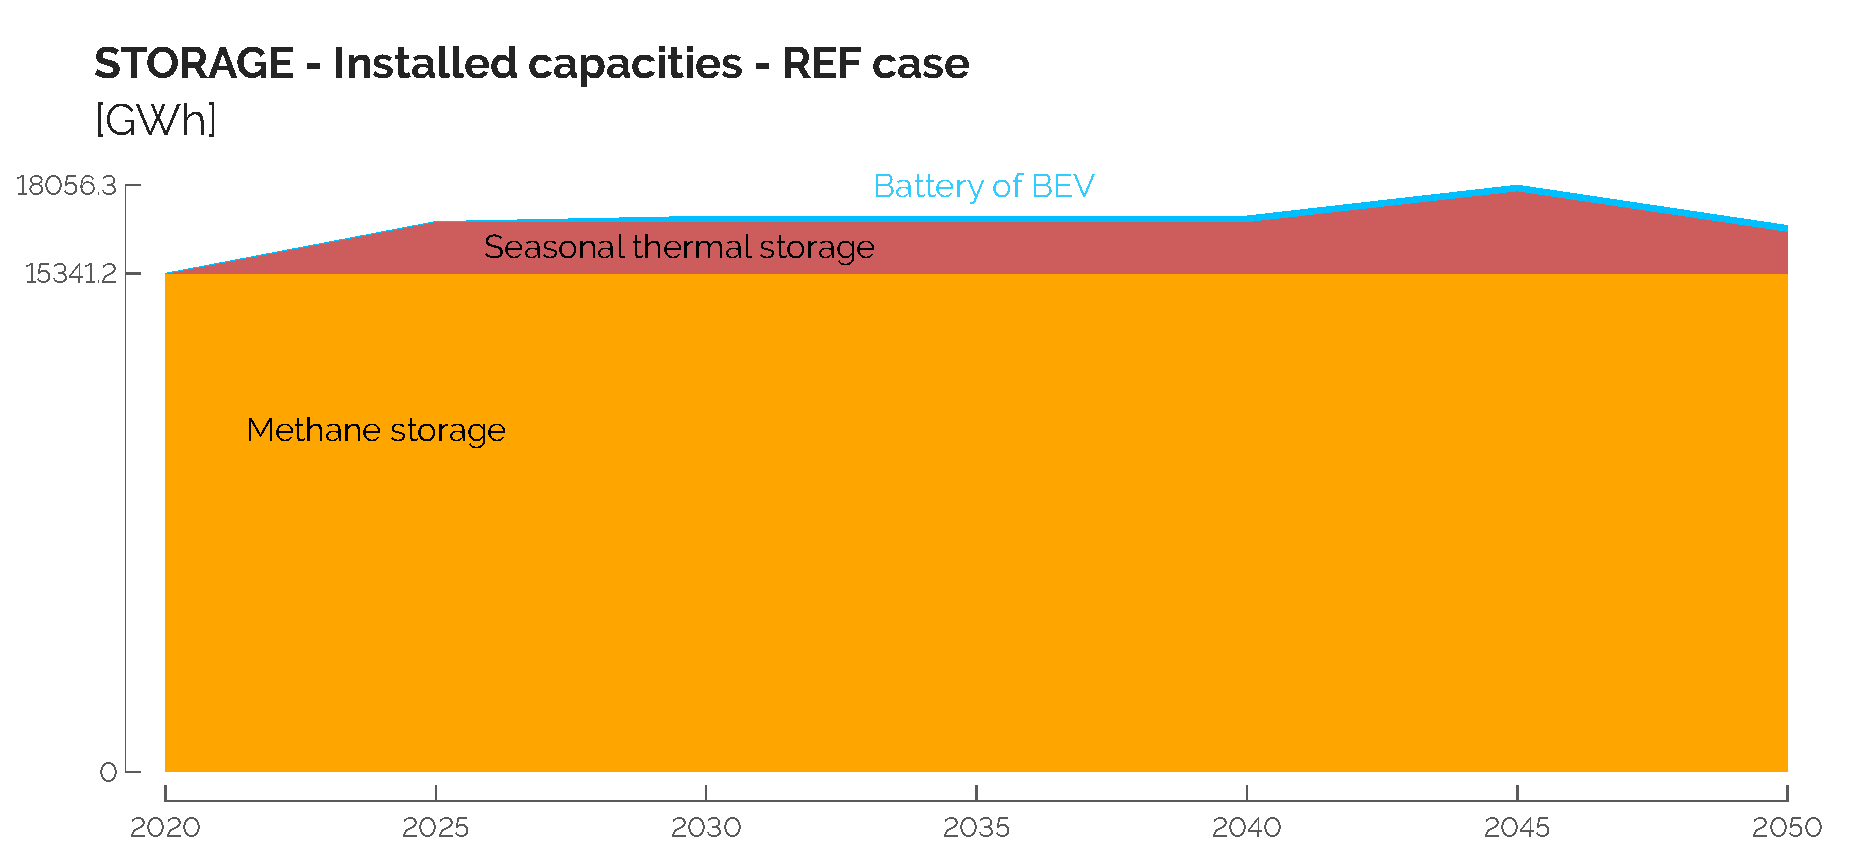
\includegraphics[width=0.7\textwidth]{STORAGE_2.pdf}
\caption{Storage installed capacities for the REF case}
\label{fig:STORAGE_2}
\end{figure}

\begin{mdframed}[style=comment] % Comment from the reviewer
{\color{teal} \textbf{Stefan}} - What is the potential of what we can learn from the results of the innovative methods? We could go further in the analysis as we know we have to phase out coal, install renewables.
\end{mdframed}

\noindent The outcome is a bit too obvious (e.g. getting rid of the coal) $\rightarrow$ go a bit in the details. Explain why the method is taking better decisions but explain why. $\rightarrow$ go beyond what we know

\begin{mdframed}[style=manuscript] % Comment from the reviewer

\end{mdframed}

\subsection{Structure}
\label{structure}

\begin{mdframed}[style=comment] % Comment from the reviewer
{\color{orange} \textbf{Stefano}} \& {\color{teal} \textbf{Stefan}} - The thesis structure makes it quite difficult to follow. Having all the methodology summarised in Chapter 1, makes it difficult to link it to the different chapters. As changing the structure may be now a major work, I would invite you to think how to better connect the different parts. 
\end{mdframed}

\noindent Initially, I wanted to group methodology and results per kind of analysis, \ie UQ on Pathway (Chapter 3), RL (Chapter 4) and PCA (Chapter 5) but that would have made the RL, and even more PCA, methodology parts come too far in the manuscript. For this reason, I made the choice to group all the methodological approaches together in Chapter 1 and the results in their respective chapters.  Given this explanation, I have added one sentence {\color{blue}at the end of the introductory paragraph of the RL method in Chapter 1}:

\begin{mdframed}[style=manuscript] % Modification to manuscript
As Chapter 2 presents the input of the case study and Chapter 3 details the results of the GSA on the pathway model, the reader interested by the results of the RL method is invited to go to Chapter 4.
\end{mdframed}

\noindent and {\color{blue}at the end of the introductory paragraph of the PCA-based method in Chapter 1}:

\begin{mdframed}[style=manuscript] % Modification to manuscript
The reader interested by the results of the PCA-based method is invited to go to Chapter 5.
\end{mdframed}

\noindent Finally, I have added a schematic at the end of the Introduction of the thesis to clarify the structure and highlight that Chapter 4 and 5 can be read after the methodological sections 1.3 and 1.4, respectively (see Figure \ref{fig:intro:Thesis_Structure}).

\begin{figure}[htbp!]
\centering
\includegraphics[width=0.7\textwidth]{Thesis_Structure.pdf}
\caption{Structure of the thesis. Beyond Chapter 2 that describes the case study of Belgium, Chapters 3, 4 and 5 collect the analyses resulting from the application of the different methodologies developed in Chapter 1. Given the (quasi-)independence of the analyses presented in the last three chapters, they can be read separately.}
\label{fig:intro:Thesis_Structure}
\end{figure}


\begin{mdframed}[style=comment] % Comment from the reviewer
{\color{violet} \textbf{Christophe}} - Formal description of the problem is missing even in described in the text to make the link between the ideas and the implementation. Add some flow charts to introduce key elements
\end{mdframed}

\noindent This point is addressed with the structure chart presented in the previous comment as well as the improvement of Figure 1.4 presenting the implementation of the myopic approach as well as the way uncertainties and RL change the values of some parameters (see Figure \ref{fig:MY_process_code} of the present document).

\subsection{References}
\label{references}

\begin{mdframed}[style=comment] % Comment from the reviewer
{\color{orange} \textbf{Stefano}} \& {\color{purple} \textbf{Sylvain}} - I found it unusual to see many references to own work (Rixhon et al.) throughout the thesis. Unless the articles are unrelated to the thesis, these references should be removed and the associated content should be included in the manuscript. As an example, at p. 25, results are mentioned which are not reported in the thesis. The reader currently must refer to [48] to see these results, which should instead be included in the thesis. 
\end{mdframed}

\noindent This choice to sometimes refer to own works was made to focus only on the main contributions of the thesis. However, I agree that some content should be included in the thesis to enhance its reading. I hereby list the references to works I have been involved in (with the reference number of the manuscript version submitted before the private defense) and detail the potential modifications brought to the manuscript for each of them.

\begin{itemize}
\item \emph{[40] Limpens et al., Energyscope pathway: an open-source model to optimise the energy transition pathways of a regional whole-energy system}: Mostly cited to give credits to Gauthier Limpens' work in developing the Pathway version of EnergyScope, I have decided to refer to the paper about the formulation choices rather than including them in the thesis manuscript. Consequently, no further modification regarding this reference.
\item \emph{[48] Limpens et al., The impact of uncertainties on the Belgian energy system: Application of the Polynomial Chaos Expansion to the EnergyScope model}: The table gathering the results of the comparison between Morris' and PCE methods has been included {\color{blue}at the end of Section 1.2.2}:
\end{itemize} 

\begin{mdframed}[style=manuscript] % Comment from the reviewer
In \cite{limpens2020impact}, we have assessed the PCE approach on the cost-optimum Belgian energy system in 2035, using EnergyScope TD. To do so, we compared the Top-14 most impacting parameters obtained from this approach with the one provided by the improved Morris method based on $\mu^*_{i}$. Even if the output of each method does not have the same physical meaning, both methods can rank the parameters by their impact on the total annual cost of the energy system. Both rankings were very similar which validated the use of PCE in the rest of this work (see Table \ref{tab:GSA:Comparison}).
\end{mdframed}

\begin{table}[htbp]
	\caption{Comparison of the Top-14 rankings for the improved Morris method (left) and total-order PCE method (right). We used the DTU's implementation of Morris method \cite{MorrisCodeDTU} (with $p=8$, $r=100$). }
    \label{tab:GSA:Comparison}
    \centering
    \begin{tabular}{lcc}
    \hline
		\textbf{Parameter} & \textbf{Morris Ranking} ($\mu^*_{i}$) & \textbf{PCE Ranking} ($S_i^T$) \\
        \hline
        Prices of hydrocarbons & 1 (0.7141) & 1 (0.6434) \\
        Cost of increased efficiency & 2 (0.3046) & 2 (0.1014) \\
        Cost of maintenance & 3 (0.2371) & 4 (0.0534) \\
        Discount rate & 4 (0.2019) & 5 (0.0467) \\
        Price of imported electricity & 5 (0.1974) & 3 (0.0809) \\
        CAPEX of the grid & 6 (0.1498) & 6 (0.0252) \\
        CAPEX of PV & 7 (0.1270) & 7 (0.0187) \\
        Increase of electricity demand & 8 (0.1168) & 8 (0.0154) \\
        CAPEX of nuclear power plant & 9 (0.0963) & 9 (0.0119) \\
        Increase of space heating demand & 10 (0.0856) & 11 (0.0088) \\
        Price of coal & 11 (0.0856) & 12 (0.0087)\\
        Price of renewable fuels & 12 (0.0794) & 10 (0.0104)\\
        Price of uranium & 13 (0.0607) & 13 (0.0047)\\
        Onshore wind load factor & 14 (0.0600) & 14 (0.0046)\\
       \hline
    \end{tabular}
\end{table}

\begin{itemize}
\item \emph{[49] Rixhon et al., The role of electrofuels under uncertainties for the Belgian energy transition}: This paper is cited to highlight the GSA performed on the snapshot model with different GWP limits. The main contribution of this work in the context of the thesis was to provide a preliminary screening and selection of parameters to carry out the GSA on the pathway model. The result of this selection is given in Section 2.4 where the uncertain parameters and their respective ranges are listed. Consequently, no further modification regarding this reference.
\item \emph{[104] Rixhon et al., Integration of non-energy among the end-use demands of bottom-up whole-energy system models}: Reference used to highlight the fact that whole-energy systems usually do not account for the non-energy demand. Consequently, no further modification regarding this reference.
\item \emph{[116] Rixhon et al., Comprehensive
integration of the non-energy demand within a whole-energy system: towards a defossilisation of the chemical industry in Belgium}: Reference to graphs that have either been adapted from the paper or directly taken from it. Consequently, no further modification regarding this reference.
\item \emph{[128] Rixhon et al., Taxonomy of the fuels in a whole-energy system}: Where the content of this paper is the Appendix A of the thesis, some references to this paper aimed at clarifying the meaning of ``renewable fuels'' (Section 2.2) or the fact that uranium is considered neither fossil nor renewable (Sections 3.1.2 and 4.2.2). Consequently, no further modification regarding this reference.
\end{itemize}



\begin{mdframed}[style=comment] % Comment from the reviewer
{\color{violet} \textbf{Christophe}} - State of the art mainly European. Why not reference to other regions of the world.
\end{mdframed}

\noindent
It is an interesting topic for further investigations, especially how they address the subject in other parts of the world like Australia/Asia. This could be linked with the political perception of energy system optimisation models and the subsequent analyses. However, no modification has been brought to the manuscript regarding this topic.

\subsection{Writing style}
\label{writing_style}

\begin{mdframed}[style=comment] % Comment from the reviewer
{\color{orange} \textbf{Stefano}} - While a more ``friendly'' writing style can be pleasant, there are many colloquial expressions that not do not fit well in the thesis, \eg ``carrot and stick'', ``apples with apples'', etc. I recommend reducing them to the bare minimum, or completely getting rid of them. 
\end{mdframed}

\noindent

\begin{mdframed}[style=manuscript] % Comment from the reviewer

\end{mdframed}

\begin{mdframed}[style=comment] % Comment from the reviewer
There are various typos in the thesis, e.g. ``storagR'' (page 3), ``therefore, therefore'' (p. 11), ``The'' (p.14), ``Moleclues'' (p. 61), etc.. Also, the use English language can be improved, e.g. ``calls FOR a variety'' (p. 9), ``cumulative emissions ARE'' (p. 14), ``than to'' (p. 34), etc. The document will benefit from a spelling/grammar check.
\end{mdframed}

\noindent The listed typos have been corrected and, overall, the manuscript has gone through Grammarly to improve the spelling and the grammar.

\subsection{Documentation}
\label{documentation}

\begin{mdframed}[style=comment] % Comment from the reviewer
{\color{purple} \textbf{Sylvain}} - Where is the repository for the code? Don't forget the documentation?
\end{mdframed}

\noindent As discussed during the private defense, this is a task that is already planned for the year to come, after the public defense. A better reference towards these repository and documentation will be given in the subsequent paper on RL. Consequently, there has not been further work done in this regard in the manuscript by the public defense.

\section{Introduction}
\label{Introduction}

\begin{mdframed}[style=comment] % Comment from the reviewer
{\color{orange} \textbf{Stefano}} \& {\color{teal} \textbf{Stefan}} - At page 1, it is mentioned that you focus on the technical levers of the transition, ``renewables'' and ``efficiency''. From this I understand that you are not focusing on ``sufficiency''. This seems to contradict a statement at p. 2, where it is mentioned that one objective of the thesis is to ``support interdisciplinary projects in the assessment of sufficiency policy''. I suggest clarifying this potential misunderstanding.  
\end{mdframed}

\noindent I totally agree with this remark, especially because I do not want to overlook the necessary third pillar of the transition which is ``sufficiency'', even though my thesis does not address directly this aspect. Consequently, I have adapted {\color{blue} page 2 of the introduction}:

\begin{mdframed}[style=manuscript] % Modification brought to the manuscript
Among all the lenses through which it is necessary to assess sufficiency policies, one of the objectives of this work is to support these interdisciplinary projects by providing informed techno-economic guidelines.
\end{mdframed}

\noindent This technical contribution to the interdisciplinary debate of sufficiency is reminded in {\color{blue} the last sentence of the conclusion}.

\begin{mdframed}[style=manuscript] % Modification brought to the manuscript
In this sense, this work provided insight about possible transition pathways for Belgium to bring the technical dimension into the intrinsically political and interdisciplinary discussions and decisions that must be made in the coming years.
\end{mdframed}

\section{Chapter 1 - Methodology}
\label{methodo}

\subsection{EnergyScope Pathway}
\label{ESPathway}
\begin{mdframed}[style=comment] % Comment from the reviewer
{\color{orange} \textbf{Stefano}} - p.11 : The stated computational time seems low for a pathway model with hourly resolution. Were there approximations (e.g., disabling crossover) added and what was their impact?\end{mdframed}

\noindent To decrease the computational time by one order of magnitude, besides opting for Gurobi to solve the LP, I disabled crossover. Besides this significant reduction of computational time, I observed no other impact regarding the values of the objective function or the design variables at the optimum. As disabling crossover is a very LP-specific aspect, I added this information {\color{blue}in a footnote in the first paragraph of Section 1.1}:

\begin{mdframed}[style=manuscript] % Modification brought to the manuscript
To keep this low computational time, crossover was disabled to solve the optimisation problem. This had no observed impact regarding the values of the objective function or the design variables at the optimum.
\end{mdframed}

\subsubsection{End-of-time-horizon}


\begin{mdframed}[style=comment] % Comment from the reviewer
{\color{orange} \textbf{Stefano}} - Often, multi-stage models are affected by the end-of-time-horizon effects. Did you observe those and how did you deal with them? See, e.g. Figure 3.3 p. 66.
\end{mdframed}

% \noindent Better highlight the importance, discuss the finetuning, discuss  alternatives (e.g. adding time windows at the end that are thrown afterwards).

\begin{mdframed}[style=manuscript] % Modification brought to the manuscript

\end{mdframed}

\subsubsection{Myopic pathway and salvage value}

\begin{mdframed}[style=comment] % Comment from the reviewer
{\color{orange} \textbf{Stefano}} - p.17-19: is the myopic version modeled as a single LP or as a sequence of LPs? This should be better clarified. The diagram at p. 19 focuses on the code, it would be better replaced by a code showcasing the logic of the approach.
\end{mdframed}

\noindent Even though this sequence of LPs was already mentioned {\color{blue}in the caption of Figure 1.3}, I have complemented the text {\color{blue} in the paragraph ``Myopic pathway implementation'' of Section 1.1.2}, 

\begin{mdframed}[style=manuscript] % Modification brought to the manuscript
[...] The myopic optimisation of the pathway consists in a sequence of smaller LP problems limited to their respective 10-year time-window, until eventually reaching 2050.
\end{mdframed}

\noindent reminded it in the caption of Figure 1.2

\begin{mdframed}[style=manuscript] % Modification brought to the manuscript
The myopic approach (in pink) uses several instances of the pathway model, illustrated in Figure 1.1, as a sequence of different and linked LP problems. 
\end{mdframed}

\noindent and extended the caption of {\color{blue} Figure 1.4}. However, besides highlighting the key step 3.3 where there is an update of parameters value, I have decided to keep the figure as is since, on the one hand, the extension of the caption provides now a better understanding and, on the other hand, the code itself is exactly what is schematically represented on the diagram. 

\begin{figure}[htbp!]
\centering
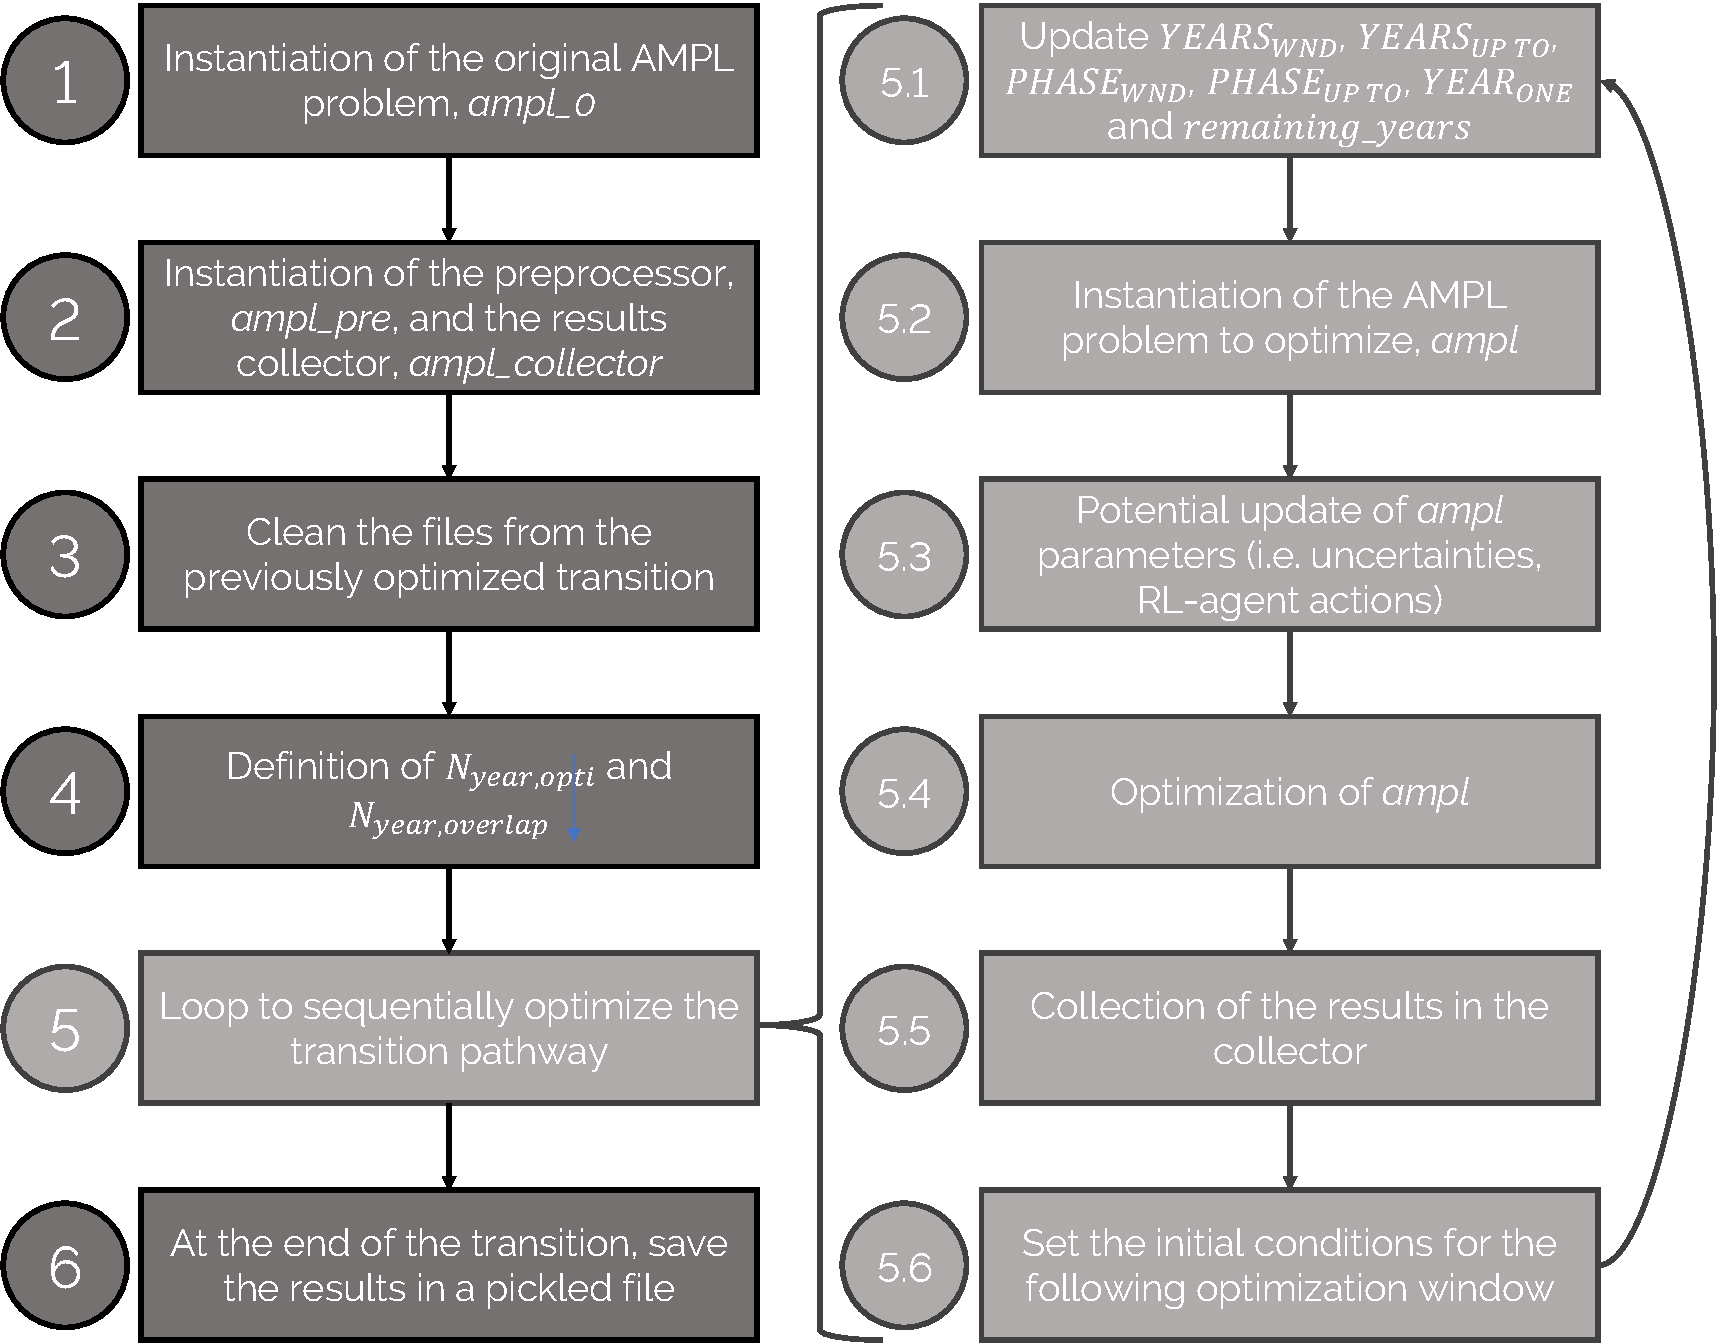
\includegraphics[width=10cm]{MY_process_code.pdf}
\caption{Diagram of the iterative optimisation of the whole-energy system transition pathway. Myopic optimisation of the pathway consists in a sequence of smaller LP problems limited to their respective 10-year time-window. If the optimisation is not deterministic, step 3.3 is the one where the value of some parameters are changed due to uncertainties (see Section 1.2) or the actions taken by the Reinforcement Learning-agent (see Chapter 4)}
\label{fig:MY_process_code}
\end{figure}

\begin{mdframed}[style=comment] % Comment from the reviewer
{\color{teal} \textbf{Stefan}} - With the myopic approach, are you predicting what will come or drawing a path that is the best? Is that a desirable feature to mimic the way we proceed now. why artificially limit the model as we know we have to go to zero in 2050.
\end{mdframed}

\noindent Link to salvage value

\begin{mdframed}[style=manuscript] % Modification brought to the manuscript

\end{mdframed}

\begin{mdframed}[style=comment] % Comment from the reviewer
{\color{teal} \textbf{Stefan}} - p.18 : Surprising that myopic leads to a sooner investment to the transition ? Is it an effect of the salvage value? was there a sensitivity analysis on this salvage value? Perhaps include more details on this. The salvage value plays a large role in the decision of the model. Give more details to give more confidence in the choice.
\end{mdframed}

\noindent Indeed, it is an effect of the salvage value as already written in the last paragraph ``Impact of myopic formulation on the system'' of Section 1.1: ``The main difference lies in the myopic transition itself and especially in the earlier
deployment of PVs and offshore wind turbines. These induce the reinforcement of the grid that is a capital-intensive and long-lifetime asset. This is mostly due to impact of the salvage value, Equation (1.4), in the objective function.''.

Sensitivity analysis has been performed on the formulation of the salvage value by \citet{goffauxpathway}. The overall conclusion of this sensitivity analysis was that the salvage value expression has little influence on the energy system at the end of the time horizon. The methodology and results of this analysis is now summed up {\color{blue}in Appendix B.2} 

\begin{mdframed}[style=manuscript] % Modification brought to the manuscript
In the work of \citet{goffauxpathway}, we carried out a sensitivity analysis on the formulation of the salvage value. First and foremost, this analysis confirmed the need to account for the salvage value to avoid penalising the capital intensive technologies towards the end of the transition \cite{poncelet2016myopic}. Then, the sensitivity analysis focused on two elements in the expression of the salvage value: $\tau_{phase}(p)$ and $\textbf{F\textsubscript{decom}}(p2,p,i)$. 

In Equation (B.22), $\tau_{phase}$ is the annualisation factor corresponding to the phase where the technology was built. With this expression, if a technology is still operational for half its lifetime after 2050, then half its initial investment is subtracted to the total transition cost. However, one could wonder if a technology that is still operational for half of its lifetime is not worth less than half of its initial investment cost, given the depreciation of the asset. In that case, the annualisation factor should account for the last phase of the optimisation (\ie 2045\_2050) when the residual value of the technologies are calculated and subtracted from the total transition cost. 

On top of this, we also investigated the impact of accounting for the decommissioned technologies or not in the expression of the salvage value.  In Equation (B.22), if a technology is decommissioned before 2050, then the salvage value of this technology will be 0. This is relevant since a technology decommissioned before 2050 would not be available after 2050. The issue is that the model could keep unnecessary technologies to subtract their salvage value from the total transition cost in order to decrease it. This would be done if the fixed OPEX of an unused technology is lower than its salvage value. Therefore, one could wonder if it would not be better to take into account the decommissioned technologies in the salvage value. In that case, a technology that would have been operational after 2050 but that had been prematurely decommissioned before 2050, would have a salvage value.

The overall conclusion of this sensitivity analysis was that the salvage value expression has little influence on the energy system at the end of the time horizon. 
\end{mdframed}

\noindent and a reference to this appendix is present {\color{blue}in Section 1.1 where Equation (1.4) is detailed}:

\begin{mdframed}[style=manuscript] % Modification brought to the manuscript
After assessing the sensitivity of the formulation of the salvage value (see Appendix B.2), we have kept the one given by Equation (1.4), being also similar to the expression used by \citet{prina2019transition}.
\end{mdframed}

\subsubsection{Discount rate and annualisation}

\begin{mdframed}[style=comment] % Comment from the reviewer
{\color{purple} \textbf{Sylvain}} - Wouldn't it be more appropriate to talk about ``discount rate'' rather than ``interest rate''?
\end{mdframed}

\noindent Indeed, as we want to capture the time preference associated with obtaining finance for the project, effectively quantifying the trade-off between present and future financial value, it is more appropriate to refer to ``discount rate'' when considering the parameter $i_{\text{rate}}$. We have changed every occurrence of ``interest rate'' into ``discount rate'' {\color{blue}in the entire manuscript}.

\begin{mdframed}[style=comment] % Comment from the reviewer
{\color{purple} \textbf{Sylvain}} - Value of the discount rate is generally above 6\% in other works. You should have a better justification of selecting 1.5\%.
\end{mdframed}

\noindent Indeed, the discount rate is usually between 7.5\% and 12\% in other studies. The main justification for this choice was to be in line with G. Limpens' work \cite{limpens2021generating}. However, assessing the impact of $i_{\text{rate}}$ on $\tau_{phase}$, we see that a lower value of $i_{\text{rate}}$ will favour less late expenses compared to a high value. In other words, considering $i_{\text{rate}}=$1.5\% rather than 10\% will less postpone investments (see Figure \ref{fig:tau_phase}). I have added some explanations in this regard {\color{blue}in Section 1.1.1}:

\begin{figure}[htbp!]
\centering
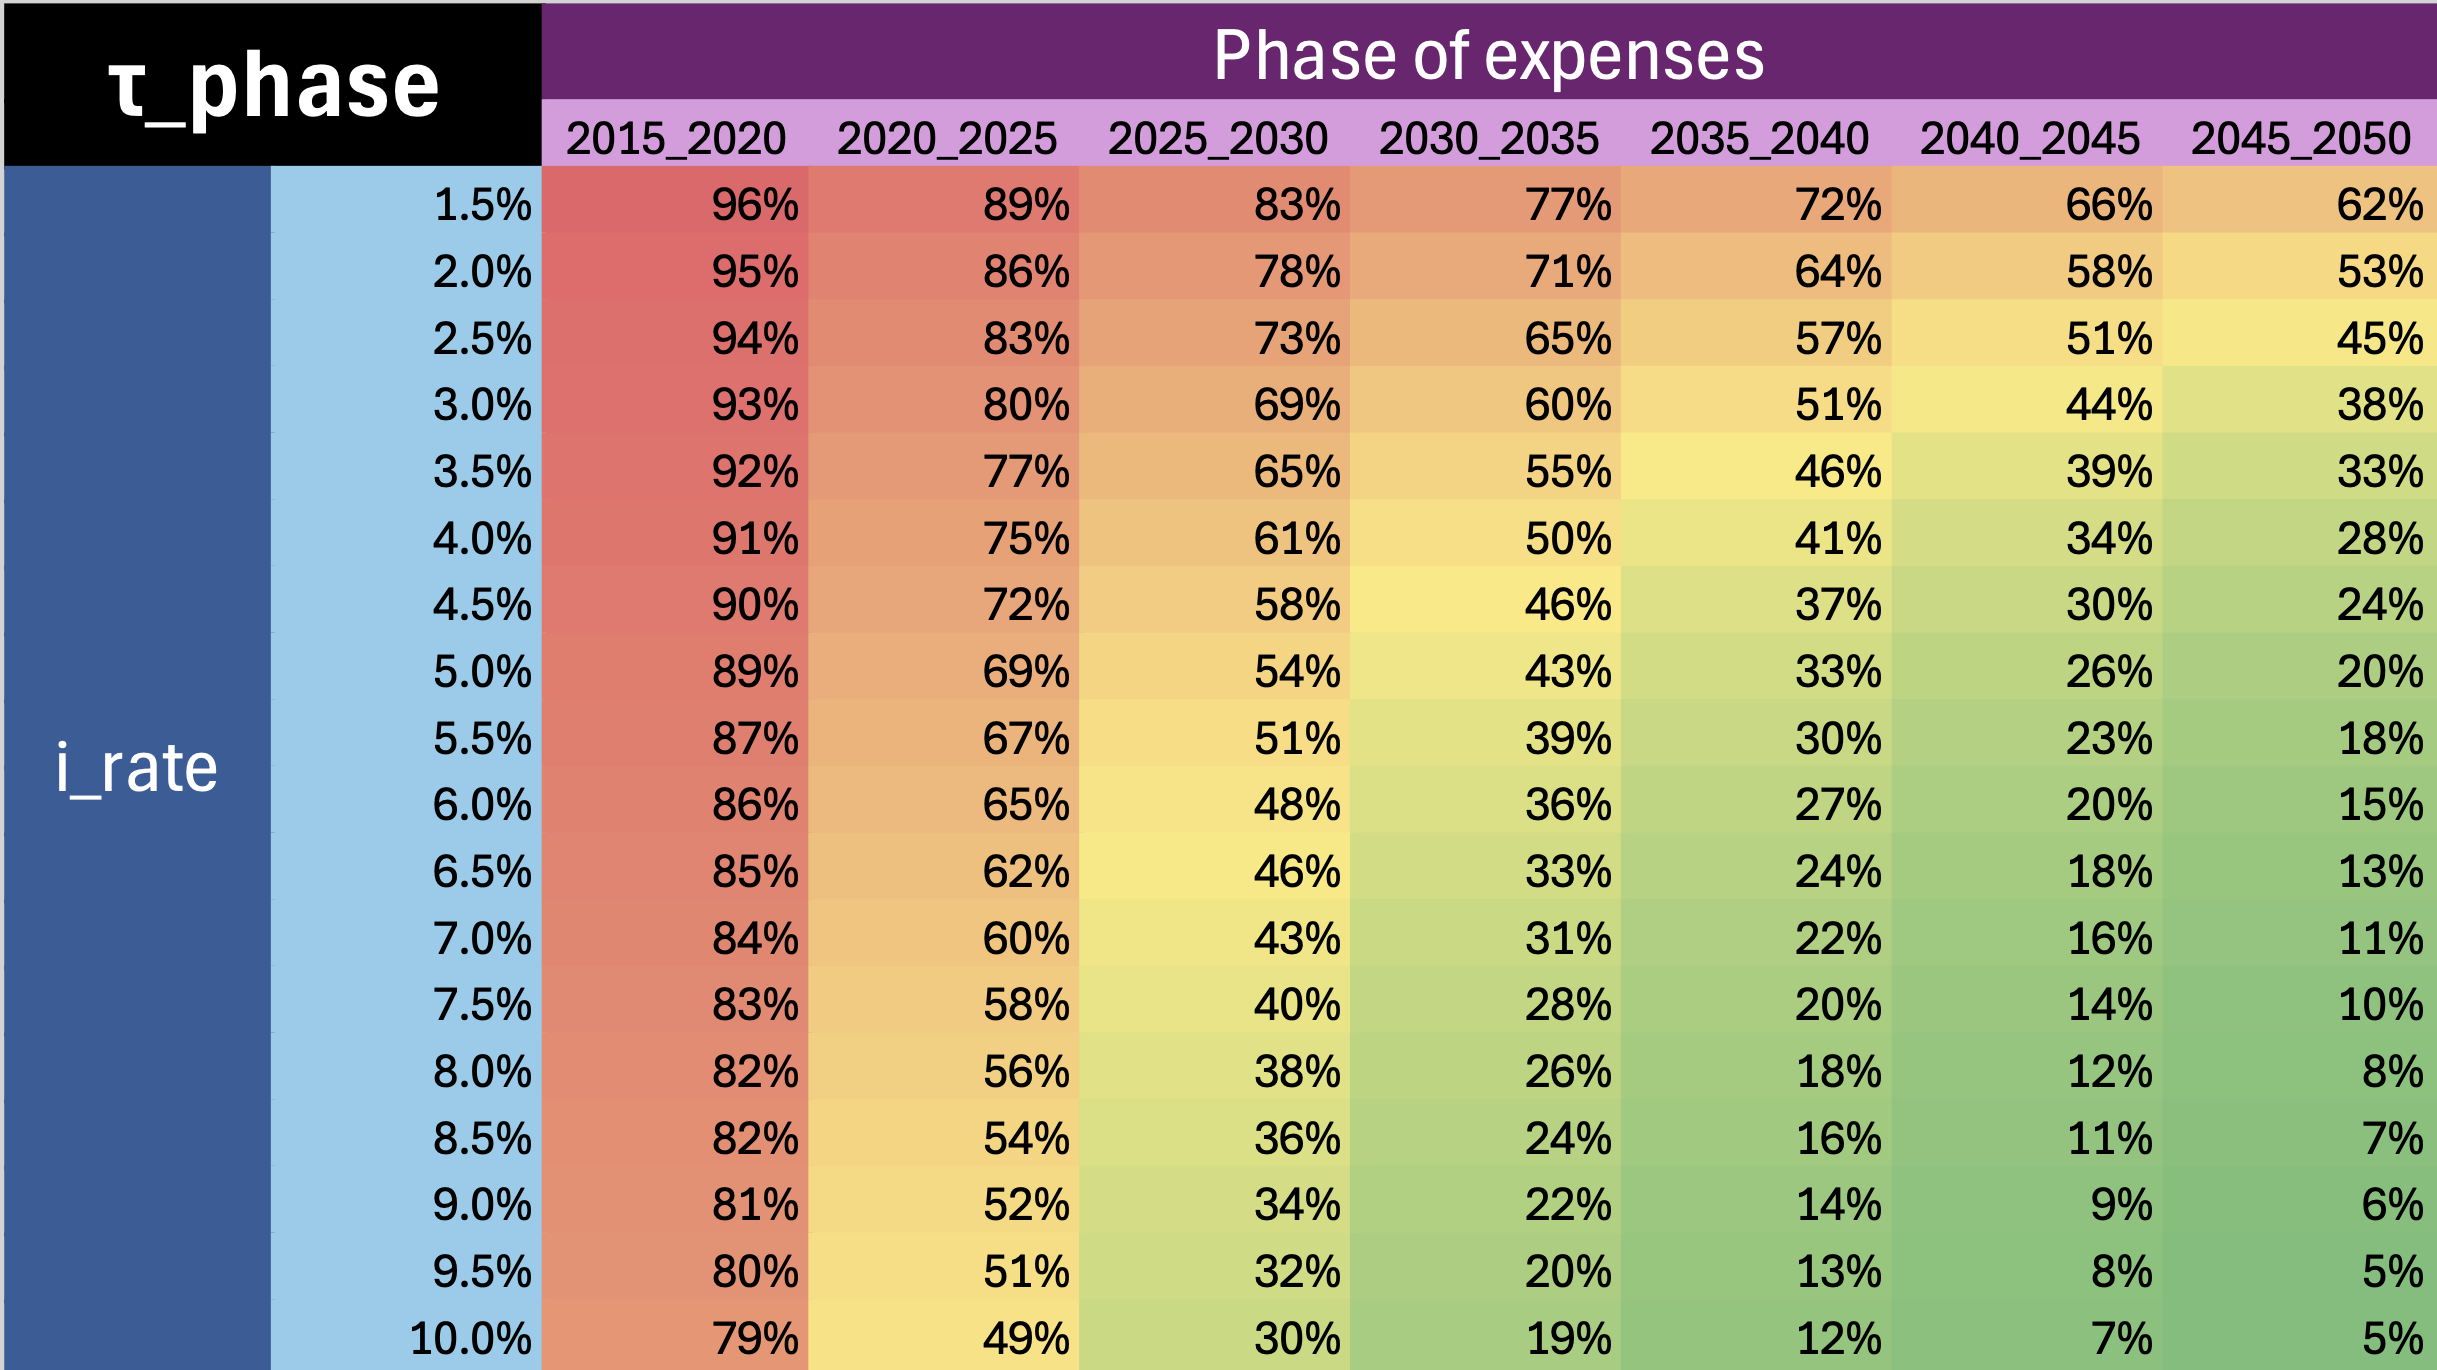
\includegraphics[width=10cm]{tau_phase.png}
\caption{$\tau_{phase}$ versus the timing of the expenses (columns) and the discount rate, $i_rate$ (rows).}
\label{fig:tau_phase}
\end{figure}



\begin{mdframed}[style=manuscript] % Modification brought to the manuscript 
In EnergyScope Pathway, $\tau\textsubscript{\emph{phase}}$ aims at depreciating the value of expenses done in the future. The discount rate accounted for in this annualisation factor, $i_{\text{rate}}$, is considered as identical for all the technologies of the system. In line with \citet{limpens2021generating}, we set the nominal value to $i_{\text{rate}}=1.5\%$ which is lower than values taken in other studies, between 7.5\% and 12\% \cite{meinke2017energy,simoes2013jrc,EuropeanCommission2016}. Having a low value of discount rate favours less late expenses compared to a higher value of discount rate.
\end{mdframed}

\begin{mdframed}[style=comment] % Comment from the reviewer
{\color{purple} \textbf{Sylvain}} - p.13: Why no annualizing over the lifetime of the unit? Would that lead to different results? 

{\color{orange} \textbf{Stefano}} - Can you explain the logic of the annualization factor in the pathway model?
\end{mdframed}

\noindent Accounting for the depreciation of money with time (see previous comment), we considered that the assets are fully paid at the moment they are installed. For this reason, we consider the arithmetic average between the investment cost of the assets at the year starting the phase of installation and the year ending it. This choice was done for two main reasons: potential decommissioning and lack of data beyond 2050. In the Pathway version of EnergyScope, the asset will be used over its whole lifetime unless it is prematurely decommissioned. Therefore, annualising over the entire lifetime of the unit might induce a bias in case of this premature decommissioning. Then, for assets with longer lifetime and/or installed later in the transition, annualising over the lifetime would require to have data beyond 2050. Effort that I have not decided to make.

Regarding the impact on the results, my educated guess is that this impact would be limited as the technologies of a same sector are assumed to have similar trends in terms of the evolution with time of their respective investment costs. Consequently, the major impact would be to end up with a lower total transition costs but the design of the system would be marginally impacted.

Given these further explanations, I have not brought any modification to manuscript in this regard.

\subsubsection{Power grid and transport infrastructure}

\begin{mdframed}[style=comment] % Comment from the reviewer
{\color{purple} \textbf{Sylvain}} - How do you model the power grid interconnections with the neighbouring countries as well as the transport network of the different energy carriers within the country?
\end{mdframed}

\noindent Copper-plate assumption $\rightarrow$ no representation of the transport sector of either electricity or gaseous and liquid energy carriers. However, one technology called ``GRID'' accounts for the additional investments in the power grid needed when deploying more VRES like PV panels and wind turbines but there is not an actual spatial representation of this grid. {\color{blue} }.

\begin{mdframed}[style=manuscript] % Modification brought to the manuscript 

\end{mdframed}

\subsection{Uncertainty quantification}
\label{methodo_UQ}

\begin{mdframed}[style=comment] % Comment from the reviewer
{\color{orange} \textbf{Stefano}} - Can you explain the choice of N=5 for the uncertainty ranges?
\end{mdframed}

\noindent

\begin{mdframed}[style=manuscript] % Modification brought to the manuscript


\end{mdframed}


\begin{mdframed}[style=comment] % Comment from the reviewer
{\color{orange} \textbf{Stefano}} - p. 20: ``inspired by Guevara et al.'' $\rightarrow$ how was their approach used in your work?
\end{mdframed}

\noindent \citet{guevara2022modeling} implemented a stochastic process to maintain realism in the evolution of uncertainty through the transition. In this sense, they avoid a parameter to go from the upper bound at year $y$ to the lower bound 5 years later. It allows zigzag from one time step to another. (see Figure \ref{fig:Guevara}). In my case, once the sample of uncertain parameters is drawn, there is no zigzag ($\alpha=0$ in \cite{guevara2022modeling}) but without especially be at the nominal value. Besides this, the inspiration does not go further. Given this explanation, I have not brought modification to the manuscript in this regard.

\begin{figure}[htbp!]
\centering
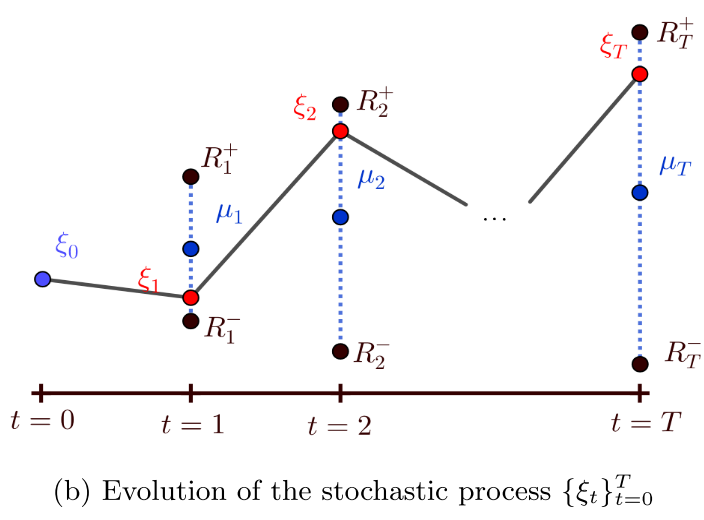
\includegraphics[width=0.5\textwidth]{Guevara.png}
\label{fig:Guevara}
\end{figure}

\begin{mdframed}[style=comment] % Comment from the reviewer
{\color{orange} \textbf{Stefano}} - p. 21: footnote. The statement is qualitative, it should be quantitative. What is the minimum number of runs needed to validate your experiments? Did you look into that? How was the surrogate model validated?
\end{mdframed}

\noindent The footnote was intentionally qualitative as the quantitative information came later on (in Section 1.2.2). To improve this, I have moved the content of this footnote into the core of the text and after this quantitative information has been brought {\color{blue}in Section 1.2.2, after ``to achieve a LOO error below 1\% for the total transition cost.''}

\begin{mdframed}[style=manuscript] % Modification brought to the manuscript
As second order PCE is the minimum to ensure accuracy of the surrogate model, selecting and grouping the parameters as presented in Section 1.2.3 is compulsory to alleviate the computational burden. Otherwise, considering thousands of independent uncertain parameters would lead to millions of EnergyScope Pathway runs, if no more. Another alternative to reduce the computational cost of the GSA would be to consider the monthly (instead of hourly) time resolution for the runs of EnergyScope Pathway. However, despite its shorter computation time (\ie couple of seconds), the main drawback of the monthly model is its poor representation of the integration of VRES \cite{limpens2024pathway}. 

\end{mdframed}

\begin{mdframed}[style=comment] % Comment from the reviewer
{\color{orange} \textbf{Stefano}} - p. 23: is PCE an appropriate method for LP / MILP models. Why is PCE needed is EnergyScope is already very fast? There is a good fit (1\% LOO error) for the total cost, which is often quite linear, but how about technology choice / sizing?
\end{mdframed}

\noindent Like in Diederik Coppitters' works \cite{coppitters2021robust,coppittersthesis}, the ``ultimate'' objective of PCE is to build up a surrogate model, $\hat{M}$, to serve a robust design optimisation (RDO) process. For an original non-linear model $M$, this surrogate model, formed of as a series of polynomials,  has the main advantage to run much faster than the original model. In my case, I used PCE as an uncertainty quantification (UQ) tool without going up to the RDO step. As written {\color{blue}in the first paragraph of Section 1.2.2}, I (only) aim at getting the statistical moments of the quantity of interest and determine Sobol' indices. Similarly, in Chapter 5, I used PCA to extract main direction of variation when it comes to the design of the system without performing runs using these PCs that are another representation of the original model. Consequently, regarding this objective, PCE is an appropriate method for EnergyScope Pathway. 

\noindent When the LOO error is higher than 1\% (but limited to 20-25\%), which is the case when performing the PCE on technology size/choice (\ie installed capacity of SMR by 2050) or the import of renewable molecules (see Section 3.2.2), the approach remains valid to qualitatively rank the parameters, {\color{blue}as discussed in the paragraph ``Qualitative ranking based on Sobol' indices'' of Section 1.2.2}.

\noindent Given these explanations and the elements already present in the text, I have not brought further modifications in the manuscript.

\begin{mdframed}[style=comment] % Comment from the reviewer
{\color{orange} \textbf{Stefano}} - p. 24: Sobol indices. Can you explain the choice wrt other methods? Difference between factor prioritization and factor fixing?
\end{mdframed}

\noindent This comparison with a similar approach like factor fixing and factor prioritization (based on Morris method \cite{morris_factorial_1991}) is detailed {\color{blue}in the paragraph ``Comparison with a proven method'' of Section 1.2.2}. I have extended this paragraph by integrating the table of comparison between the Morris method and PCE.  This also avoids the reference to our own work and the reference [48], page 25 (see previous comment).

\noindent Besides being an in-house used method, the choice to use PCE is to be able to quickly extract statistical moments of the output of interest, as explained {\color{blue}in the first paragraph of Section 1.2.2}.

\begin{mdframed}[style=comment] % Comment from the reviewer
{\color{purple} \textbf{Sylvain}} - p.21 - How are the groups of uncertainties defined? Is there a table?
\end{mdframed}

\noindent Even though the uncertain parameters, their groups and their ranges of uncertainties might be the same for other case studies, they have been especially adapted for the present case study, \ie Belgium. Consequently, I decided to exhaustively list these uncertain parameters in the chapter dedicated to the case study (see Section 2.4). However, to not leave the reader handing there and wondering if there other parameters and how we have decided to group them, I have added a reference to Section 2.4 {\color{blue}at the end of Section 1.2.1} focusing on the characterisation of the uncertainties:

\begin{mdframed}[style=manuscript] % Modification brought to the manuscript 
Section 2.4 gathers the list of the uncertain parameters considered in this work.
\end{mdframed}

\begin{mdframed}[style=comment] % Comment from the reviewer
{\color{purple} \textbf{Sylvain}} - Table 1.2 - what are the other parameters?
\end{mdframed}

\noindent See previous comment.

\subsection{Reinforcement Learning}
\label{methodo_RL}

\begin{mdframed}[style=comment] % Comment from the reviewer
{\color{orange} \textbf{Stefano}} - p. 31: Can you explain the need of using NN here? Couldn’t you just run the energyscope model?
\end{mdframed}

\noindent 

\begin{mdframed}[style=manuscript] % Modification brought to the manuscript

\end{mdframed}

\begin{mdframed}[style=comment] % Comment from the reviewer
{\color{purple} \textbf{Sylvain}} - p. 27 When presenting the advantages of RL, you mention model-free approach. Ok, but you have a representation of the real world available to train the model!
\end{mdframed}

\noindent {\color{blue} }.

\begin{mdframed}[style=manuscript] % Modification brought to the manuscript 

\end{mdframed}

\begin{mdframed}[style=comment] % Comment from the reviewer
{\color{teal} \textbf{Stefan}} - Justification of the actions selected? why no other actions like the cost of some technologies? 
\end{mdframed}

\noindent These actions have a direct translation in constraints and we can therefore assess their effectiveness through the fact they are binding or not. Give examples of actions tried during the work (incentivize renewables) or other from Assemblée citoyenne in France and explain why they’re not as good as those chosen in the thesis. Explain history of what we tried/consider? 
 {\color{blue} }.

\begin{mdframed}[style=manuscript] % Modification brought to the manuscript 

\end{mdframed}

\subsection{Principal Component Analysis}
\label{methodo_PCA}

\begin{mdframed}[style=comment] % Comment from the reviewer
{\color{orange} \textbf{Stefano}} - p. 32: Why is PCA needed? Wouldn’t it be easier to just aggregate similar outputs of interest?
\end{mdframed}

\noindent 

\begin{mdframed}[style=manuscript] % Modification brought to the manuscript

\end{mdframed}

\begin{mdframed}[style=comment] % Comment from the reviewer
{\color{orange} \textbf{Stefano}} - p. 42: Figure 1.17. What is your definition of robustness? Having a tight distribution but all shifted towards very suboptimal costs seems to fit your definition. Please clarify.
\end{mdframed}

\noindent 

\begin{mdframed}[style=manuscript] % Modification brought to the manuscript

\end{mdframed}

\begin{mdframed}[style=comment] % Comment from the reviewer
{\color{purple} \textbf{Sylvain}} - p. 39 Why are their outliers in the first case? Isn't a bit arbitrary to set them to a min/max value?
\end{mdframed}

\noindent I should insist on those elements in the text {\color{blue} }.

\begin{mdframed}[style=manuscript] % Modification brought to the manuscript 

\end{mdframed}

\section{Chapter 2 - Case study}
\label{case_study}

\subsection{General and introduction}
\label{methodo_general}

\begin{mdframed}[style=comment] % Comment from the reviewer
{\color{orange} \textbf{Stefano}} - I am a bit underwhelmed by the many nitty-gritty data in this Chapter. While it is surely important to document everything, couldn’t at least part of this be moved to the Appendix?\end{mdframed}

\noindent 

\begin{mdframed}[style=manuscript] % Modification brought to the manuscript

\end{mdframed}

\begin{mdframed}[style=comment] % Comment from the reviewer
{\color{purple} \textbf{Sylvain}} - p. 45 How is the range accounted for the characterisation of private mobility technologies?
\end{mdframed}

\noindent Indeed, the increase of the range is a consequence of the increased efficiency and battery capacity. Consequently, I have removed the mention to the range {\color{blue}at the end of the last paragraph in the contributions of Chapter 2}.

\begin{mdframed}[style=manuscript] % Modification brought to the manuscript 
Regarding BEV, while the CAPEX has been kept unchanged, the efficiency and the battery capacity have been increased. 
\end{mdframed}

\subsection{End-use demands}
\label{methodo_eud}

\subsection{Resources}
\label{methodo_resources}

\begin{mdframed}[style=comment] % Comment from the reviewer
{\color{purple} \textbf{Sylvain}} - p. 51 Last paragraph of p. 51 is not clear. Are we talking about the purchase cost or the CO2 content?
\end{mdframed}

\noindent There was indeed a confusion in the information to deliver in this paragraph. For the sake of clarity, I have restructured Section 2.2. After the introductory paragraph, the graphs and the following paragraph focus on the cost of purchasing. The two last paragraphs address the aspects of availabilities and global warming potentials, respectively.

\subsection{Conversion technologies}
\label{methodo_technologies}

\begin{mdframed}[style=comment] % Comment from the reviewer
{\color{orange} \textbf{Stefano}} - Figure 2.5: What is the purpose of the violet line between ``biomass gasification'' and ``methanolation''?
\end{mdframed}

\noindent These were actually two different arrows, one pointing from ``biomass gasification for CH3OH'' to ``Methanol'' and the other from ``Methanolation'' to ``Methanol''. To avoid this confusion, the figure has been updated and the origin of these arrows are now on different vertical levels ({\color{blue} see Section 2.3}).

\begin{figure}[htbp!]
\centering
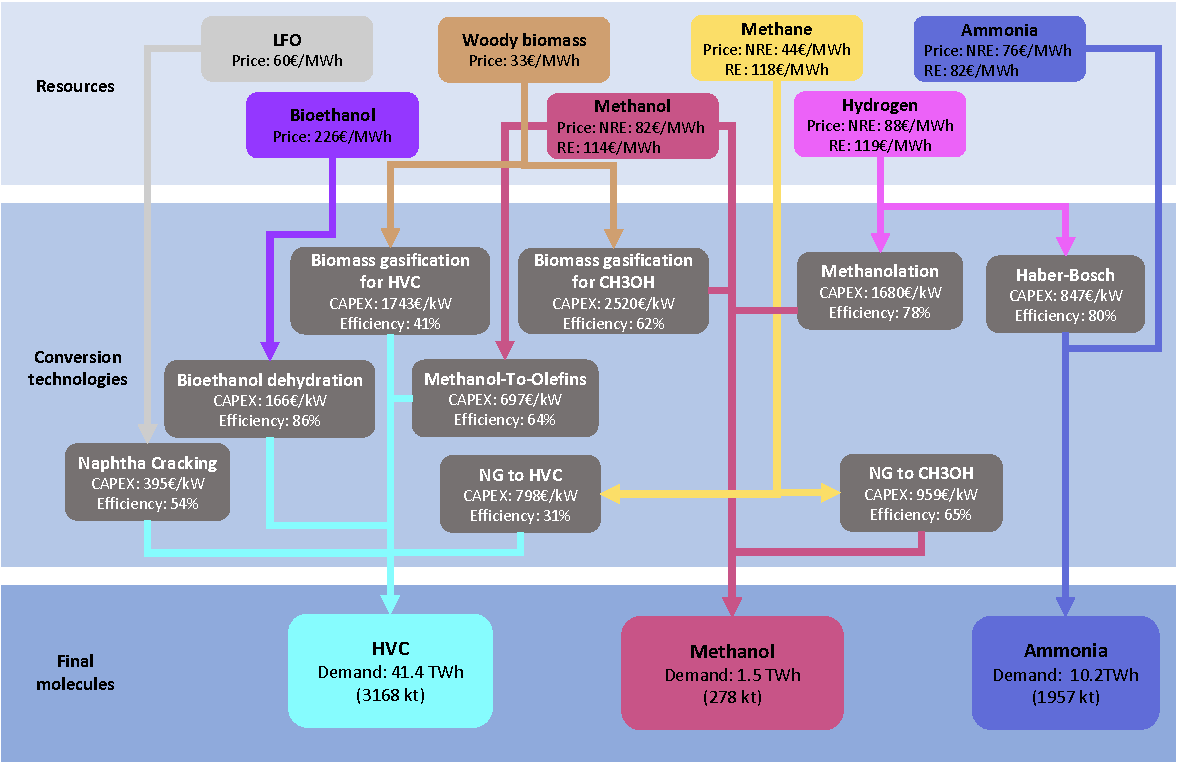
\includegraphics[width=\textwidth]{NED_tech.pdf}
\label{fig:NED_tech}
\end{figure}

\begin{mdframed}[style=comment] % Comment from the reviewer
{\color{purple} \textbf{Sylvain}} - p. 54 Is there a differentiation between ground mounted and rooftop PV?
\end{mdframed}

\noindent In the continuity of Gauthier Limpens' works \cite{limpens2021generating}, we consider here only rooftop PV. This potential of 59.2\,GW corresponds to 250 km$^2$ of available roof well oriented that exist today. Accounting for ground mounted PV would almost double this potential, as shown in Paolo Thiran's thesis. In future works, it would be interesting to also implement this additional potential, especially for the sake of harmonisation of input data. On the contrary, Elia, the Belgian TSO, foresees a much more limited increase of installed PV, \ie 18\,GW by 2034 \cite{Elia_2024_2034}. Consequently, for this thesis, I have decided to stick to this intermediate potential of 59.2\,GW. For the sake of clarity, I only added ``rooftop'' {\color{blue}in the second paragraph of Section 2.2}:

\begin{mdframed}[style=manuscript] % Modification brought to the manuscript 
On the other hand, wind, solar, hydro and uranium are limited by the technical potentials of rooftop PV panels (59.2\,GW) [...]
\end{mdframed}

\begin{mdframed}[style=comment] % Comment from the reviewer
{\color{purple} \textbf{Sylvain}} - p. 51: Offshore wind max capacity is too low and PV is lower than Bregilab.
\end{mdframed}

\noindent Concerning the potential of PV, see previous comment. Regarding offshore wind, we have assumed a conservative potential of 6\,GW as the lower bound of the forecast done by the Belgian offshore platform\footnote{https://www.belgianoffshoreplatform.be/fr/}. Similarly to EnergyVille \cite{PATHS2050}, we could have gone up to the upper bound of 8\,GW. Going much higher, such as 24\,GW for the ``Electrification'' scenario of EnergyVille, would account for access to a part of the 150\,GW offshore wind park project in the North Sea signed betwee Belgium, Germany, Denmark and the Netherlands (the ``Esbjerg Offshore Wind Declaration''). 

\noindent Since these potentials have been discussed and detailed in previous works and are not the main topic of my thesis, I have not brought any further modification to the manuscript in this regard.

\begin{mdframed}[style=comment] % Comment from the reviewer
{\color{purple} \textbf{Sylvain}} - p. 51 Why investigating SMR?
\end{mdframed}

\noindent As discussed during the private defense, we have decided to investigate to role of nuclear energy in the future for two main reasons: hot topic in Belgium and similar study by EnergyVille \cite{PATHS2050}. First, when presenting the results of our work at conferences/meetings, we have been asked many times how our results, massively relying on imports of renewable molecules, were influenced by the installation of nuclear power plants by 2050. Second, during my thesis, EnergyVille delivered a report PATHS2050 where, among others, they investigated the impact of SMR. As they observed that installing SMR would significantly reduce the need to import renewable molecules, we also wanted to assess this impact in our work. Given these explanations, no further modification has been brought to the manuscript in this regard.

\begin{mdframed}[style=comment] % Comment from the reviewer
{\color{purple} \textbf{Sylvain}} - p. 53 4850€/kW is at the lower end of the EnergyVille scenario for SMR (4500€/kW). This is a very optimistic price forecast! Current tenders for 3rd generation are higher than 100€/MWh. There are papers showing that SMRs are not really expected to be cheaper than 3rd generation. How realistic is 41 €/MWh? LCOE of SMRs would be much higher if: - the capital cost was more realistic and, - the Capacity factor was lowered to account for their flexible use.
\end{mdframed}

\noindent As discussed during the private defense, similarly to EnergyVille \cite{PATHS2050}, we have considered the same CAPEX for SMR as the one considered for conventional nuclear power plants. Where EnergyVille considers a nominal CAPEX of 7500€/kW (like the current large Gen III design of Hinkley Point in the UK), we considered 4850€/kW like the CAPEX of conventional nuclear units in EnergyScope. 

On top of the uncertainty applied to the CAPEX of SMR [-40\%, 44\%] considered in the thesis, I carried out a test on these assumptions by plotting the LCOE of electricity-production units considering different assumptions for SMR (see Figure \ref{fig:LCOE_comparison}). Even considering 50\% more expensive SMR subject to a higher discount rate (5\% versus 1.5\% for the other technologies), we notice that SMR keeps on being more cost-competitive than other flexible production units, like e-ammonia CCGTs, that are substituted by SMR when the latter can be installed (see Chapter 3). In other words, it means that the optimistic values assumed for SMR in the thesis lead to a cheaper whole-energy system but does not affect its design, \ie the installed technologies.  Consequently, no further modification has been brought to the thesis regarding this comment.

\begin{figure}[htbp!]
\centering
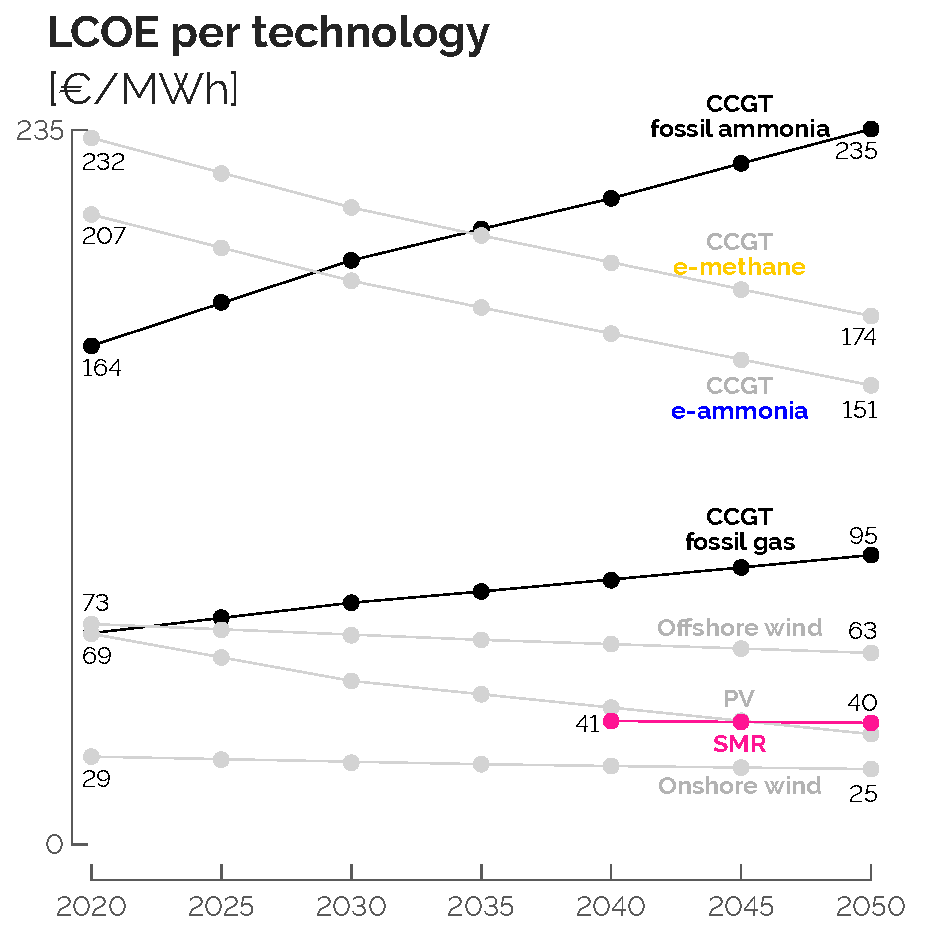
\includegraphics[width=0.49\textwidth]{LCOE_line_2.pdf}
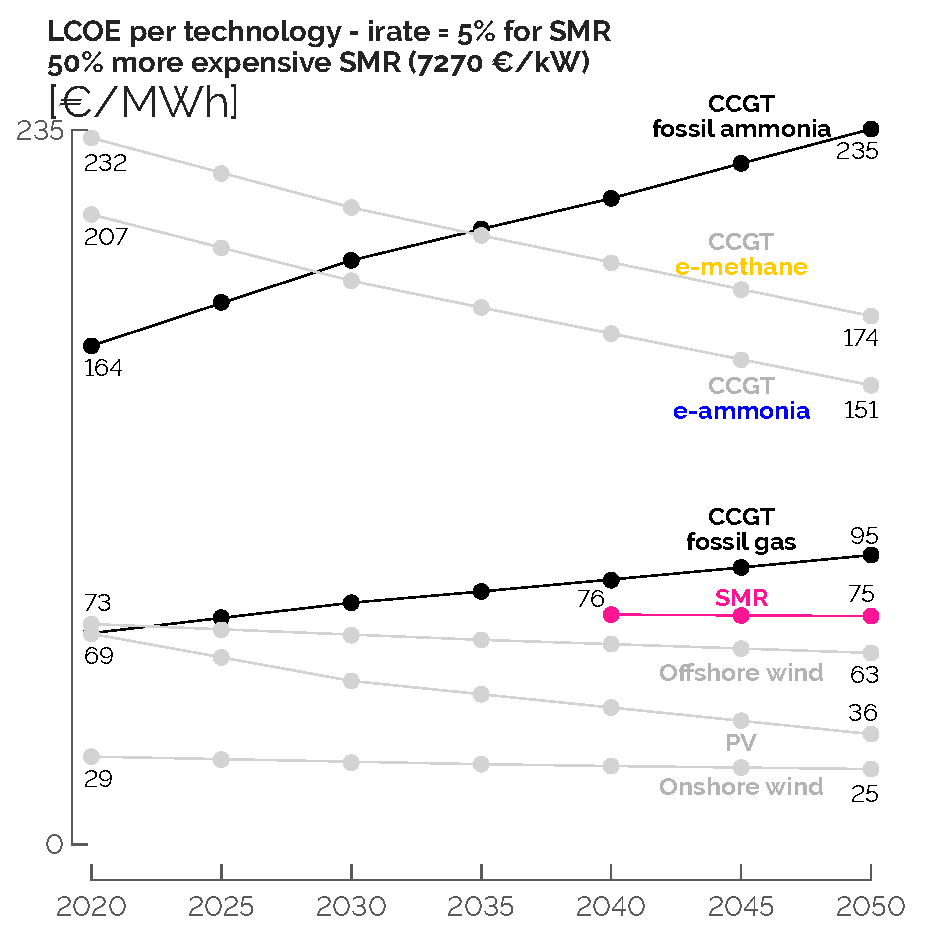
\includegraphics[width=0.49\textwidth]{LCOE_line_3.pdf}
\label{fig:LCOE_comparison}
\caption{LCOE per technology producing exclusively electricity considered in the thesis (left) and same LCOE but, this time, with a higher CAPEX (7270€/kW versus 4850€/kW in the thesis and a discount rate of 5\% on this technology. Even considering these less favourable assumptions for SMR, it still outcompetes other flexible production units like CCGT running on e-ammonia.}
\end{figure}

\begin{mdframed}[style=comment] % Comment from the reviewer
{\color{purple} \textbf{Sylvain}} - p. 53 What about fuel cost?
\end{mdframed}

\noindent Even though the cost of purchasing uranium was already presented in Figure 2.3 of the thesis, I have added this value {\color{blue}in Table 2.1}:

\begin{table}[htbp!]
\caption{Nominal features of the SMRs in EnergyScope. SMR exhibits the advantage to have a fully flexible production (\ie between 0 to the full capacity) unlike conventional nuclear that is constrained to produce a constant baseload at every hour of the year.}
\label{tab:SMR_features}
\begin{minipage}{\linewidth}
\centering
\begin{tabular}{l c c}
\hline
\textbf{Feature} & \textbf{Value} & \textbf{Unit}\\
\hline
CAPEX & 4850 & €/kW \\
Annual OPEX & 103 & €/kW/year \\
Lifetime & 60 & year \\
\textbf{Cost of purchasing uranium} & \textbf{4} & \textbf{€/MWh}\\
Efficiency & 40\% & -\\
Maximum capacity & 6 & GW \\
Annual availability & 85\% & -\\
Operational year & 2040 & - \\
Flexibility & Full & - \\
\hline						

\end{tabular}
\end{minipage}
\end{table}

\begin{mdframed}[style=comment] % Comment from the reviewer
{\color{purple} \textbf{Sylvain}} - p. 55 - Figure 2.5 - Coupled with heat for endogenous and exogenous reactions?
\end{mdframed}

\noindent Indeed, the potential consumption/production of heat and/or electricity for each conversion process is considered in the model. For instance, the Methanol-To-Olefins (MTO) process consumes 1.24\,GWh of methanol and 0.33\,GWh of high-temperature heat to produce 1\,GWh of HVC, which makes a 64\% efficiency. To clarify this point, {\color{blue}the caption of Figure 2.5} has been extended:

\begin{mdframed}[style=manuscript] % Modification brought to the manuscript 
Schematic view of the different resources able to produce HVC, ammonia and methanol with their related conversion technologies (including energy efficiency and their CAPEX - in €/kW of final molecules).  \textbf{The efficiencies account for the potential consumption/production of heat and/or electricity within each conversion process.} Values stand for 2035. Graph from \cite{rixhon2021comprehensive}.
\end{mdframed}

\begin{mdframed}[style=comment] % Comment from the reviewer
{\color{purple} \textbf{Sylvain}} - p. 56 Are modal shares exogenously set?
\end{mdframed}

\noindent In line with \citet{limpens2019energyscope}, modal shares are indeed exogenously set. This aims at keeping some realism and ensures the need of less cost-competitive options like private versus public transport or decentralised versus DHN heating. To clarify this point, it is now explicitly written {\color{blue}in Section 2.4}:

\begin{mdframed}[style=manuscript] % Modification brought to the manuscript 
[...] (ix) other parameters like the discount rate or the \textbf{exogenous} modal share change in different key sectors.
\end{mdframed}

\begin{mdframed}[style=comment] % Comment from the reviewer
{\color{purple} \textbf{Sylvain}} - p. 57: Why a uniform distribution? A gaussian would clearly be more appropriate. Maybe some uncertainties are underestimated (because clipped by uniform distribution).
\end{mdframed}

\noindent As already written in the first paragraph of Section 1.2.1, given the scarcity of data to actually define a distribution of uncertainty for the parameters, the common practice is to consider uniform distribution. As detailed by \citet{coppittersthesis}: ``Distributions are typically defined based on large datasets, which are not always at hand for each parameter. Therefore, when no meaningful information can be extracted on the distribution from a limited dataset, a uniform distribution is typically assumed, which assigns an equal probability to each value within a range. This approach is similar to assigning an interval to a parameter, but takes advantage of the central tendency when uniform distributions are propagated through a system model (\ie central limit theorem)''. Given what is already in the thesis manuscript and these further explanation, no modification has been brought to the manuscript in this regard. 

\section{Chapter 3 - Atom-vs-molecules}
\label{Chap_atom_vs_molecules}

\begin{mdframed}[style=comment] % Comment from the reviewer
{\color{orange} \textbf{Stefano}} - Would it be fair to say that the scope of this Chapter is adding one technology (SMR) to the model? Is this a significant contribution?
\end{mdframed}

\noindent Besides having added SMR to the model which is one of the contributions regarding the case study (Chapter 2), the main contributions of this chapter is the global sensitivity analysis (GSA) performed on the optimisation of the transition pathway of a whole-energy system with 34 uncertain parameters. When applied to the case study of Belgium, this analysis also allowed to highlight the competition between SMR and some of the imported electrofuels (mostly e-ammonia and e-methane) by 2050. 

To make it clearer from the beginning of the Chapter, I have extended {\color{blue}the contributions of Chapter 3}:

\begin{mdframed}[style=manuscript] % Modification brought to the manuscript
This GSA applied to a model optimising the transition pathway of a whole-energy system with these many uncertain parameters is the main contribution of this chapter. Through this analysis, we also managed to point out the impact of integrating SMR in the Belgian energy system as well as the main drivers of the import of e-hydrogen, e-methane, e-ammonia and e-methanol by 2050.
\end{mdframed}

\begin{mdframed}[style=comment] % Comment from the reviewer
{\color{orange} \textbf{Stefano}} - What is the learning of this chapter? I was underwhelmed by the long list of results. What is the take-away?
\end{mdframed}

\noindent The results are deeply detailed in Sections 3.1 and 3.2. These sections address the impact of adding SMR in the deterministic solution (\ie uncertain parameters at their respective nominal value) of the Belgian energy transition and global sensitivity analyses on different outputs of interest, respectively.  The purpose of these two sections is to give numerical substance to the main conclusions and take-aways that are listed in Section 3.3:
\begin{itemize}
\item If available, SMR is installed and mostly affect the electricity and high-temperature sectors;
\item To minimise the variation of the total transition cost, the key parameter is the cost of purchasing electrofuels where parameters related to SMR (availability and CAPEX) have much lower impact;
\item E-ammonia and, to a lesser extent, e-methane imports by 2050 are impacted by the availability of SMR whereas e-hydrogen and e-methanol are rather influenced by variation related to transport technologies and non-energy demand, respectively;
\item Even though SMR and electrofuels are in competition, they do not limit the deployment of VRES in Belgium. In other words, investing in wind and solar is a must-do for the Belgian energy transition;
\item Given the set of assumptions, especially considering the end-use-demands and the local potential of VRES, Belgium will need to import molecules in the near future. On top of investing into VRES, it seems reasonable to invest in the imports of these electrofuels as betting on SMR means letting the short-term emissions go up and, potentially, requiring significant (and quick) adjustments in case the technology is not ready on time to still respect the \ce{CO2}-budget.
\end{itemize}

Given these explanations and what is already written in the manuscript, I have not brought further modification to the manuscript in this regard.

\begin{mdframed}[style=comment] % Comment from the reviewer
{\color{orange} \textbf{Stefano}} - p. 70: ``in other words, the variation of the parameter $f_{\mathrm{max,SMR}}$…''. I am not sure that this sentence is equivalent to the previous one. Please clarify.
\end{mdframed}

\noindent The Sobol' index is the ratio between the variance of the total transition cost due to the variation of one parameter and the total variance of the total transition cost. If $f_{\mathrm{max,SMR}}$ takes a value between 0 and 0.59, the impact on the system, and, consequently, on its total transition cost, is the same: no SMR installed. A wide range of variation of the parameter leading to zero variation of the output of interest is one of the reasons to explain why the Sobol' index of this parameter is low. To clarify this point, I have rephrased the sentence {\color{blue}in Section 3.2.1}:

\begin{mdframed}[style=manuscript] % Modification brought to the manuscript
Given the uncertainty characterisation presented in Section 2.4, there are 60\% chance that no SMR could be installed. \textbf{When $f_{\mathrm{max,SMR}}$ takes a value between 0 and 0.59, the variation of the total transition cost is only due to the variation of the other parameters. }
\end{mdframed}

\begin{mdframed}[style=comment] % Comment from the reviewer
{\color{orange} \textbf{Stefano}} - p. 71, Table 3.1: isn’t the low impact simply due to the low assumed potential? Is this finding meaningful?
\end{mdframed}

\noindent This low assumed potential is indeed one of the reasons why the SMR-related uncertain parameters have a limited impact on the total transition cost as already stated in the first paragraph of Section 3.2.1: ``However, given its limited deployment, up to 6\,GW, SMR-related parameters have a lower impact on the variation of the total transition cost.''. However, this is not the only reasons as detailed earlier in the same paragraph: the late potential availability (2040 at the soonest) as well as the ``cheap and low-emitting fuel, the long lifetime leading to lower annualised CAPEX and higher salvage value.''. 

Given these explanations and what is already written in the manuscript, I have not brought further modification to the manuscript in this regard.

\begin{mdframed}[style=comment] % Comment from the reviewer
{\color{orange} \textbf{Stefano}} - p. 74, Figure 3.8: this graphs looks potentially interesting but it is not sufficiently well explained.
\end{mdframed}

\noindent The objective of this set of figures is to point out the key parameters that drive the variation of some outputs of interest. Taking the case of Figure 3.8, we focus on the import of e-methanol in 2050. On the x-axis, we represent the value taken by the uncertain parameters in the different samples. As the range is not the same for all the parameters, we have limited this axis from ``Min'' to ``Max''. The y-axis represents the feature of interest. The drawn lines represent average trend lines between the output of interest and one specific parameter. For the case of Industry EUD, for samples of the GSA where this uncertain parameter is at 35\% of its range, the mean value of methanol imported in 2050 is roughly 50\,TWh. The distributions present on the extreme left and right of the graphs correspond to the distributions of the output of interest for the samples of the GSA where the considered parameter takes a value in the bottom (left) or top (right) 15\% of its range. 

To improve the readability of this figure, I have updated the text zones to specify that these lines and distributions represent results of some specific samples of the GSA. Additionally, I have added a text zone to remind that the value between brackets is the Sobol' index of the considered parameter regarding this specific output of interest, and added this information in the caption of the figure:

\begin{figure}[htbp!]
\centering
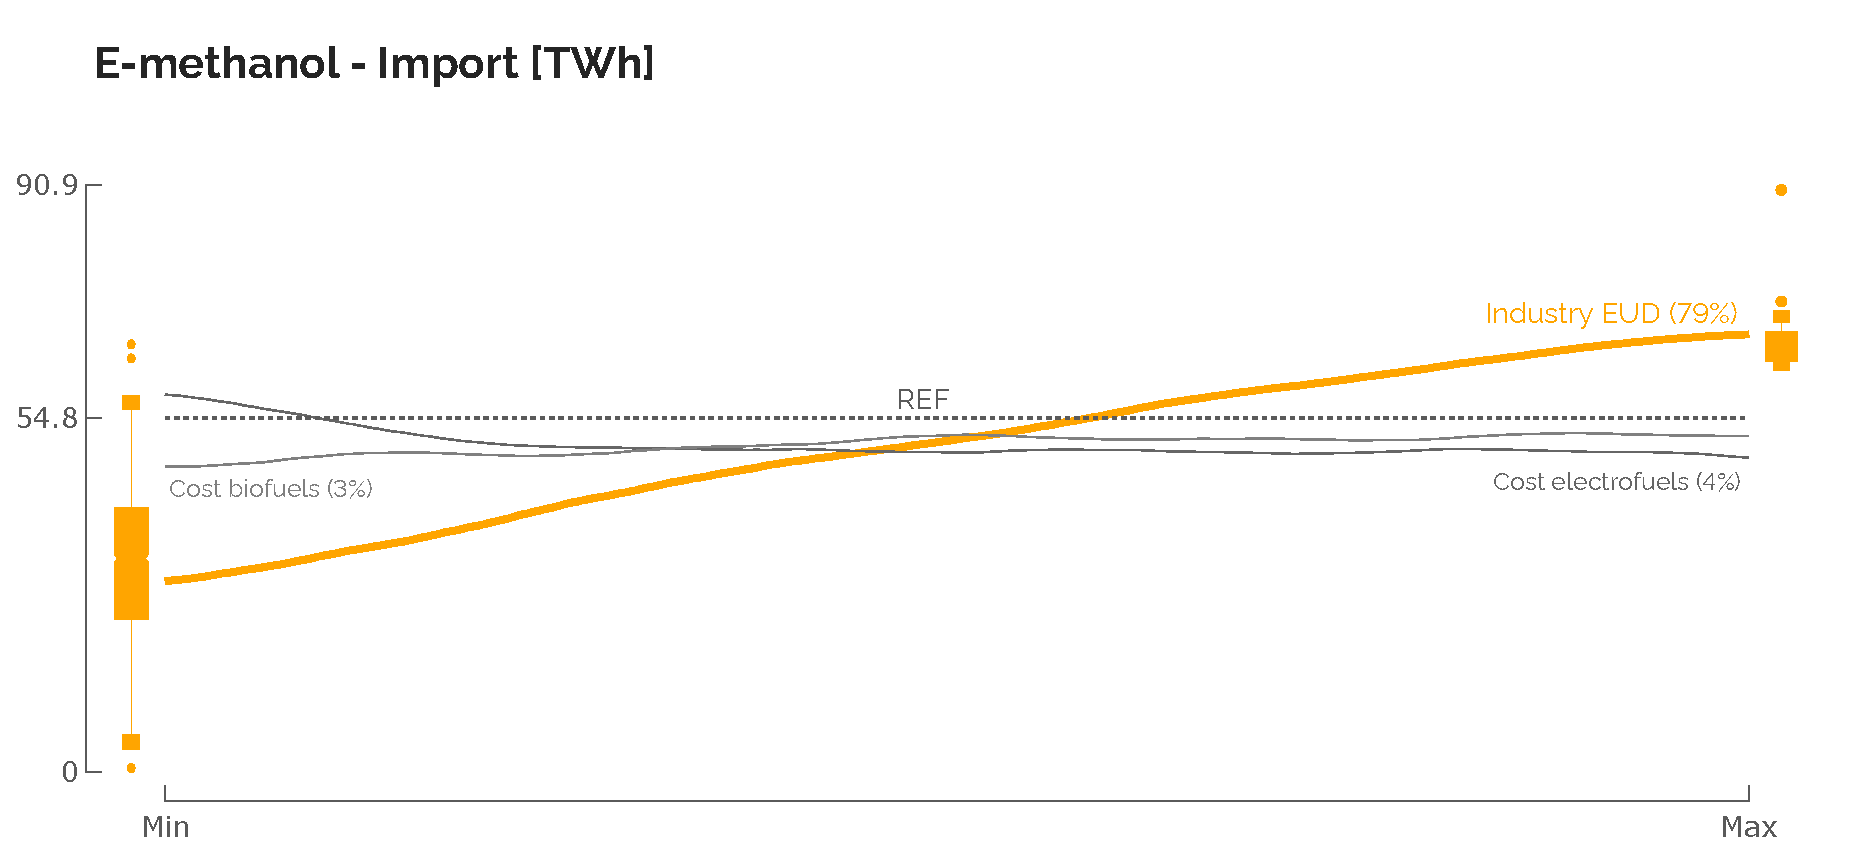
\includegraphics[width=0.8\textwidth]{UQ_Methanol_samples_2.pdf}
\caption{Trend lines of the key parameters (and their Sobol' index) on the import of e-methanol in 2050. Around these lines, box plots point out the distribution of the output of interest for the extreme values (either bottom-15\% or top-15\%) of some parameters. The grey dashed line gives the value of the output of interest in the REF case. }
\label{fig:results_uq_samples_methanol}
\end{figure}


\begin{mdframed}[style=comment] % Comment from the reviewer
{\color{purple} \textbf{Sylvain}} - p. 63 What does efficiency change in the installed capacity?
\end{mdframed}

\noindent Indeed, the efficiency only has an impact on the amount of primary uranium needed to produce the electricity. Consequently, I have removed this part of the sentence {\color{blue}in the first paragraph of Section 3.1.1}. 

\begin{mdframed}[style=manuscript] % Modification brought to the manuscript 
Overall, given the restriction on yearly availability and the slightly higher electrification [...]
\end{mdframed}

\begin{mdframed}[style=comment] % Comment from the reviewer
{\color{purple} \textbf{Sylvain}} - p. 64 - 15 GW of PV in 2025. Realistic?
\end{mdframed}

\noindent {\color{blue} }. 

\begin{mdframed}[style=manuscript] % Modification brought to the manuscript 

\end{mdframed}

\begin{mdframed}[style=comment] % Comment from the reviewer
{\color{purple} \textbf{Sylvain}} - p. 65 - Decides to use ammonia instead of SNG => is the transport infrastructure accounted for?
\end{mdframed}

\noindent {\color{blue} }. 

\begin{mdframed}[style=manuscript] % Modification brought to the manuscript 

\end{mdframed}

\begin{mdframed}[style=comment] % Comment from the reviewer
{\color{purple} \textbf{Sylvain}} - p. 67 - It really depends on what is considered primary energy in the case of nuclear
\end{mdframed}

\noindent As specified in the table about SMR features (see previous comment), the considered fuel for SMR is uranium, as it is the case for conventional nuclear power plants. Given this, I have not brought modification to the manuscript in this regard.

\begin{mdframed}[style=comment] % Comment from the reviewer
{\color{purple} \textbf{Sylvain}} - p. 69 - No curtailment at all? It would be nice to have the exact number.
\end{mdframed}

\noindent {\color{blue} }. 

\begin{mdframed}[style=manuscript] % Modification brought to the manuscript 

\end{mdframed}

\begin{mdframed}[style=comment] % Comment from the reviewer
{\color{purple} \textbf{Sylvain}} - p. 69 - Very strange. Should be the same as for industrial boilers. No smart charging?
\end{mdframed}

\noindent {\color{blue} }. 

\begin{mdframed}[style=manuscript] % Modification brought to the manuscript 

\end{mdframed}

\begin{mdframed}[style=comment] % Comment from the reviewer
{\color{purple} \textbf{Sylvain}} - p. 70 - But that's because the CAPEX is way too low. With more realistic values, the Sobol would be much higher.
\end{mdframed}

\noindent {\color{blue} }. 

\begin{mdframed}[style=manuscript] % Modification brought to the manuscript 

\end{mdframed}

\begin{mdframed}[style=comment] % Comment from the reviewer
{\color{purple} \textbf{Sylvain}} - p.71 - Differentiated discount rates could be useful.
\end{mdframed}

\noindent As written in Chapter 3: ``In practice, the discount rate would vary depending on the technology investment risk''. Depending on the technology readiness level, private investors would be more or less risk-averse. However, EnergyScope only considers a vision of a central-planner where a single agent makes the investment decisions without differentiating the sources of the capitals, \ie private and public. Assuming a differentiated discount rate would require to make assumptions about the private-public distribution of the capitals. These further explanations for keeping a single value of discount rate have been added {\color{blue} after Eq. (1.3) when discussing the annualised phase factor}.

\begin{mdframed}[style=manuscript] % Modification brought to the manuscript 
The discount rate accounted for in the annualisation factor is considered as identical for all the technologies of the system. In practice, the discount rate would vary depending on the technology investment risk. Depending on the technology readiness level, private investors would be more or less risk-averse. However, EnergyScope only considers the vision of a central-planner where a single agent makes the investment decisions without differentiating the sources of the capitals, \ie private and public. Assuming a differentiated discount rate would require to make assumptions about the private-public distribution of the capitals. For this reason, we have decided to keep an identical value of discount rate for all the technologies.
\end{mdframed}

\begin{mdframed}[style=comment] % Comment from the reviewer
{\color{purple} \textbf{Sylvain}} - p. 72 - Battery trucks are gaining momentum. Is the hydrogen route really the way to go?
\end{mdframed}

\noindent {\color{blue} }. 

\begin{mdframed}[style=manuscript] % Modification brought to the manuscript 

\end{mdframed}

\begin{mdframed}[style=comment] % Comment from the reviewer
{\color{purple} \textbf{Sylvain}} - p. 73 - How is the transport infrastructure accounted for?
\end{mdframed}

\noindent {\color{blue} }. 

\begin{mdframed}[style=manuscript] % Modification brought to the manuscript 

\end{mdframed}

\begin{mdframed}[style=comment] % Comment from the reviewer
{\color{purple} \textbf{Sylvain}} - p. 78 - Why this threshold? Shouldn't it follow the potential capacity?
\end{mdframed}

\noindent {\color{blue} }. 

\begin{mdframed}[style=manuscript] % Modification brought to the manuscript 

\end{mdframed}

\begin{mdframed}[style=comment] % Comment from the reviewer
{\color{teal} \textbf{Stefan}} - Lot of the results hinge on the import of e-fuels with the assumption that they have GWP = 0; is it justified? Those fuels are directly available knowing they are no.
\end{mdframed}

\noindent Perhaps reinforce the message as you answered the question $\rightarrow$ We need to go for radical changes, a “unicorn” solution, and one option would be the import of renewable molecules {\color{blue} }. 

\begin{mdframed}[style=manuscript] % Modification brought to the manuscript 

\end{mdframed}



\begin{mdframed}[style=comment] % Comment from the reviewer
{\color{teal} \textbf{Stefan}} - SMR / interest rate must be revisited if a paper is published.
\end{mdframed}

\noindent {\color{blue} }. 

\begin{mdframed}[style=manuscript] % Modification brought to the manuscript 

\end{mdframed}

\section{Chapter 4 - Reinforcement Learning}
\label{Chap_RL}


\begin{mdframed}[style=comment] % Comment from the reviewer
{\color{orange} \textbf{Stefano}} - Explain more in details the different steps in the RL approach
\end{mdframed}

\noindent 

\begin{mdframed}[style=manuscript] % Modification brought to the manuscript

\end{mdframed}

\begin{mdframed}[style=comment] % Comment from the reviewer
{\color{orange} \textbf{Stefano}} - p. 84: Why -300? Seems like fine-tuned to obtain desired results?
\end{mdframed}

\noindent 

\begin{mdframed}[style=manuscript] % Modification brought to the manuscript

\end{mdframed}

\begin{mdframed}[style=comment] % Comment from the reviewer
{\color{orange} \textbf{Stefano}} - p. 85, Figure 4.1: Does it mean we can run ``infinite energy transitions''? Is this realistic? Isn’t the ``learning'' supposed to happen during the different stages?
\end{mdframed}

\noindent 

\begin{mdframed}[style=manuscript] % Modification brought to the manuscript

\end{mdframed}

\begin{mdframed}[style=comment] % Comment from the reviewer
{\color{orange} \textbf{Stefano}} - How can you account for pivotal events / shocks in the system?
\end{mdframed}

\noindent 

\begin{mdframed}[style=manuscript] % Modification brought to the manuscript

\end{mdframed}

\begin{mdframed}[style=comment] % Comment from the reviewer
{\color{orange} \textbf{Stefano}} - p. 89: Figure 4.3 seems to deliver an important message (early action is needed to ensure we meet climate goals), but it is not clearly explained. Improve captions / add axes. 	Where do I see the ``tipping points'' in this figure?
\end{mdframed}

\noindent 

\begin{mdframed}[style=manuscript] % Modification brought to the manuscript

\end{mdframed}

\begin{mdframed}[style=comment] % Comment from the reviewer
{\color{orange} \textbf{Stefano}} - Overall, I suggest adding a diagram to Chapter 4, detailing what are the actions available to the decision-maker.
\end{mdframed}

\noindent 

\begin{mdframed}[style=manuscript] % Modification brought to the manuscript

\end{mdframed}

\begin{mdframed}[style=comment] % Comment from the reviewer
{\color{orange} \textbf{Stefano}} \& {\color{purple} \textbf{Sylvain}} - How does this approach compare, for example, to stochastic programming?
\end{mdframed}

\noindent This work will be done for the subsequent paper on RL. The strategy would to implement a simplified case study (\ie smaller system, fewer uncertain parameters and more limited time horizon) where it would be ``computationally more affordable'' to test the stochastic programming approach and compare it with the optimal policy delivered by the RL approach. Consequently, regarding this comment, there has not been further modification brought to the manuscript.

\begin{mdframed}[style=comment] % Comment from the reviewer
{\color{orange} \textbf{Stefano}} - p. 90: What does it mean to succeed/fail in 2030? And why are the number of attempts reduced going down in the graph?
\end{mdframed}

\noindent 

\begin{mdframed}[style=manuscript] % Modification brought to the manuscript

\end{mdframed}

\begin{mdframed}[style=comment] % Comment from the reviewer
{\color{orange} \textbf{Stefano}} - p.91, Table 4.2: how do you differentiate between actions that depend on the agent and exogenous uncertainties? More in general: how is uncertainty integrated in the RL framework?
\end{mdframed}

\noindent 

\begin{mdframed}[style=manuscript] % Modification brought to the manuscript

\end{mdframed}

\begin{mdframed}[style=comment] % Comment from the reviewer
{\color{orange} \textbf{Stefano}} - p. 94: Figure 4.6 seems to be less revealing than other figures. Also the figure caption seems to contradict the first statement following the figure. It would be important to clarify: which are the actions that emerge to actually matter?
\end{mdframed}

\noindent 

\begin{mdframed}[style=manuscript] % Modification brought to the manuscript

\end{mdframed}

\begin{mdframed}[style=comment] % Comment from the reviewer
{\color{purple} \textbf{Sylvain}} - p. 86 - A lot of heuristic and trial and error. Can the methodology be generalized to other models?
\end{mdframed}

\noindent {\color{blue} }. 

\begin{mdframed}[style=manuscript] % Modification brought to the manuscript 

\end{mdframed}

\begin{mdframed}[style=comment] % Comment from the reviewer
{\color{purple} \textbf{Sylvain}} - p. 87 - What is a step?
\end{mdframed}

\noindent To define in Section 1.3.2 and remind here {\color{blue} }. 

\begin{mdframed}[style=manuscript] % Modification brought to the manuscript 

\end{mdframed}

\begin{mdframed}[style=comment] % Comment from the reviewer
{\color{purple} \textbf{Sylvain}} - p. 96 - The early constraints on generation avoid lock-in situations correct?
\end{mdframed}

\noindent {\color{blue} }. 

\begin{mdframed}[style=manuscript] % Modification brought to the manuscript 

\end{mdframed}

\begin{mdframed}[style=comment] % Comment from the reviewer
{\color{purple} \textbf{Sylvain}} - p. 96 - Why 10 years if the step is 5?
\end{mdframed}

\noindent To explain in the definition of the action {\color{blue} }. 

\begin{mdframed}[style=manuscript] % Modification brought to the manuscript 

\end{mdframed}

\begin{mdframed}[style=comment] % Comment from the reviewer
{\color{teal} \textbf{Stefan}} \& {\color{purple} \textbf{Sylvain}} - p. 97 - The agent can reach systems that are cheaper than any other solution obtained by the perfect foresight approach. How can this be possible?
\end{mdframed}

\noindent {\color{blue} }. 

\begin{mdframed}[style=manuscript] % Modification brought to the manuscript 

\end{mdframed}

\begin{mdframed}[style=comment] % Comment from the reviewer
{\color{purple} \textbf{Sylvain}} - p. 100 - What/where are the no-go zones? Is there a narrative to describe them ?
\end{mdframed}

\noindent  {\color{blue} }. 

\begin{mdframed}[style=manuscript] % Modification brought to the manuscript 

\end{mdframed}

\begin{mdframed}[style=comment] % Comment from the reviewer
{\color{violet} \textbf{Christophe}} - The concept of binding constraint was not clear.
\end{mdframed}

\noindent
Besides the information given in Section 4.2.3 of the manuscript (and reminded here below), I do not see further explanations that could clarify the concept of binding constraint in a Linear Programming (LP) problem. Consequently, regarding this comment, there has not been further modification brought to the manuscript.

\begin{mdframed}[style=manuscript] % Modification brought to the manuscript
To identify the actions that have an actual impact on the environment, we can check if they are binding or not. In a LP problem, constraints represent hyperplanes in the domain of variables. In a two-dimension space, these are straight lines (see Figure 4.7). When the problem is bounded and feasible, these lines are the edges of a convex polygon: the domain of feasibility. The optimal solution, $\textbf{x}^*$, is the combination of variables leading to the optimal value of the objective function. Besides being within the domain of feasibility, it is proven that this optimal solution, when unique\footnote{There are cases where the objective function has the same optimal value along an entire edge. In this case, there is an infinity of solutions and the problem is indeterminate.}, locates on a vertex of the domain \cite{bertsimas1997introduction}. The constraints intersecting at this vertex are considered as binding, actually limiting the objective function to be more optimal. In other words, binding constraints, when tightened, aggravate the objective value function. If these are inequality constraints, as represented in Figure 4.7, it means that their left and right sides of the equation are equal.
\end{mdframed}

\section{Chapter 5 - Principal Component Analysis}
\label{PCA}

\begin{mdframed}[style=comment] % Comment from the reviewer
{\color{orange} \textbf{Stefano}} - p. 101: you mention different definitions of “robustness”: which one do you use in your work?
\end{mdframed}

\noindent 

\begin{mdframed}[style=manuscript] % Modification brought to the manuscript

\end{mdframed}

\begin{mdframed}[style=comment] % Comment from the reviewer
{\color{orange} \textbf{Stefano}} - p. 109: how is Gamma-robustness implemented here? It seems like it is in some sense “manually” forced? Explain better how the ROB solution is derived.
\end{mdframed}

\noindent 

\begin{mdframed}[style=manuscript] % Modification brought to the manuscript

\end{mdframed}

\begin{mdframed}[style=comment] % Comment from the reviewer
{\color{violet} \textbf{Christophe}} When using the word ``component'', there seems to be a confusion and it is not always easy to understand if you refer to the vector or the coefficient related to one of the original variable.
\end{mdframed}

\noindent The confusion probably comes from the fact a Principal Component (PC) actually represents an eigenvector of the covariance matrix. This vector is, by definition, composed of \textbf{components}, each of them being a coefficient related to a specific original variable. Parts where the word ``component'' is not directly linked to ``vector'', ``eigenvector'' or ``PC'' are those that could mislead the reader. Modifications have been brought to these parts.

{\color{blue} End of second paragraph of section 1.4.1}:

\begin{mdframed}[style=manuscript] % Modification brought to the manuscript
Moreover, this means that \textbf{the coefficient} $\alpha_{ki}$, \ie the component of $\bm{\alpha}_{\mathbf{k}}$ related to the $i^{\text{th}}$ original variable, $x_i$,  gives its weight in the $k^{\text{th}}$ PC, \ie $z_k$. 
\end{mdframed}

\section{Conclusion}
\label{Conclusion}

\begin{mdframed}[style=comment] % Comment from the reviewer
{\color{orange} \textbf{Stefano}} \& {\color{purple} \textbf{Sylvain}} - p. 119: the statement mentioning the ``major added value of the perfect foresight'' approach seems surprising and needs to be clarified. 
\end{mdframed}

\noindent 

\begin{mdframed}[style=manuscript] % Modification brought to the manuscript

\end{mdframed}

\begin{mdframed}[style=comment] % Comment from the reviewer
{\color{teal} \textbf{Stefan}} - The conclusion is a summary and should rather be a discussion (\eg discard coal as soon as possible is obvious).
\end{mdframed}

\noindent To explain in the definition of the action {\color{blue} }. 

\begin{mdframed}[style=manuscript] % Modification brought to the manuscript 

\end{mdframed}


\clearpage
\def\bibfont{\scriptsize}
\bibliography{../bib_thesis.bib}
\normalsize

\end{document}